\section{Search Algorithms}
\label{sec:search-algorithms}

This section describes the development of distributed algorithms that enable a group of robots to collaboratively search a map for a target object. All algorithms are implemented in the \texttt{botbrain} library.

\subsection{The Roomba Algorithm}
The Roomba algorithm serves as a baseline for evaluating the performance of more advanced behaviors. This simple obstacle avoidance algorithm moves in a straight line until the robot encounters an obstacle, at which point it turns away until it can resume moving forward. \\

In its implementation, the robot uses LiDAR data to locate the nearest obstacle. If the obstacle is within a predefined safety threshold, the robot rotates away. The resulting paths from this behavior are shown in \cref{fig:roomba-paths}.

\def\w{0.329\textwidth}
\begin{figure}[H]
    \centering
    \begin{subfigure}[b]{\w}
        \centering
        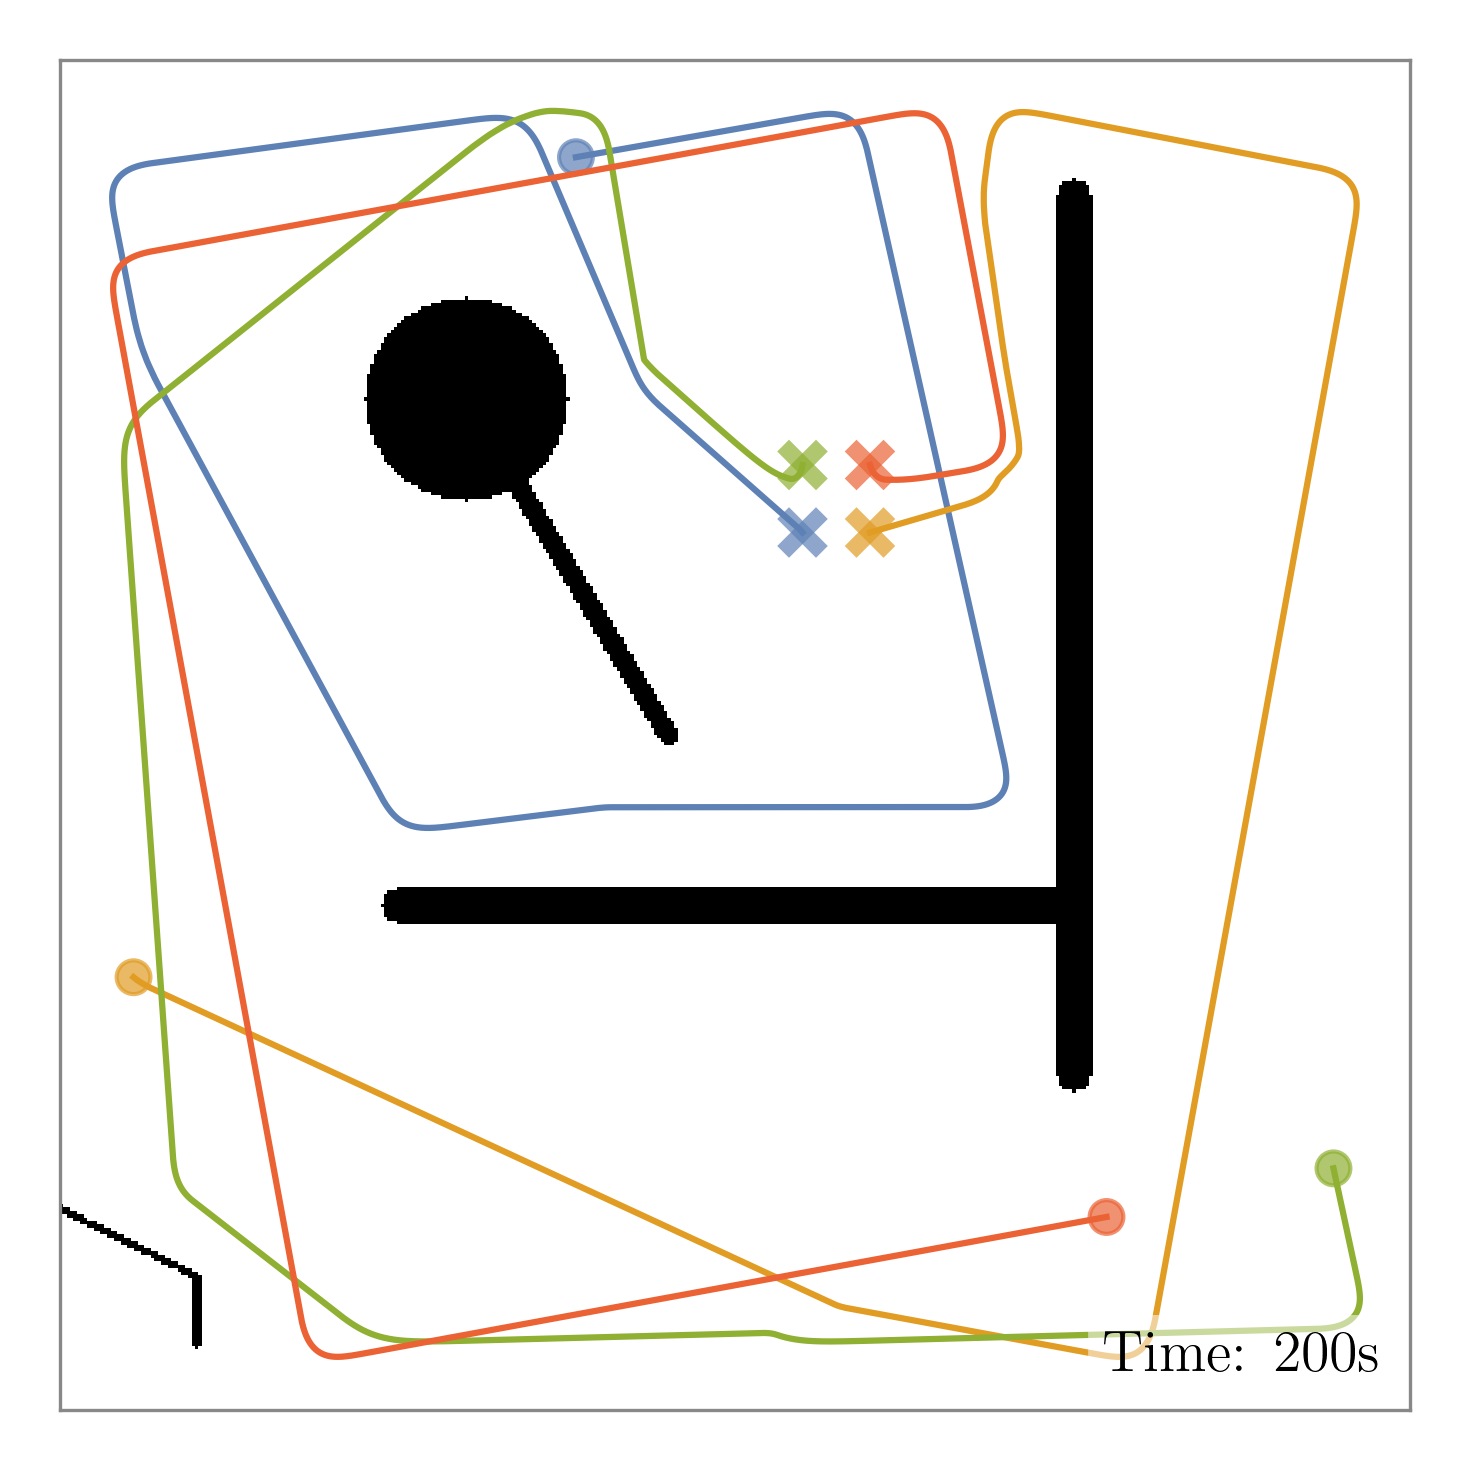
\includegraphics[width=\textwidth]{./figures/plots/paths/avoid-obstacles-paths-(after-200s).png}
    \end{subfigure}
    \begin{subfigure}[b]{\w}
        \centering
        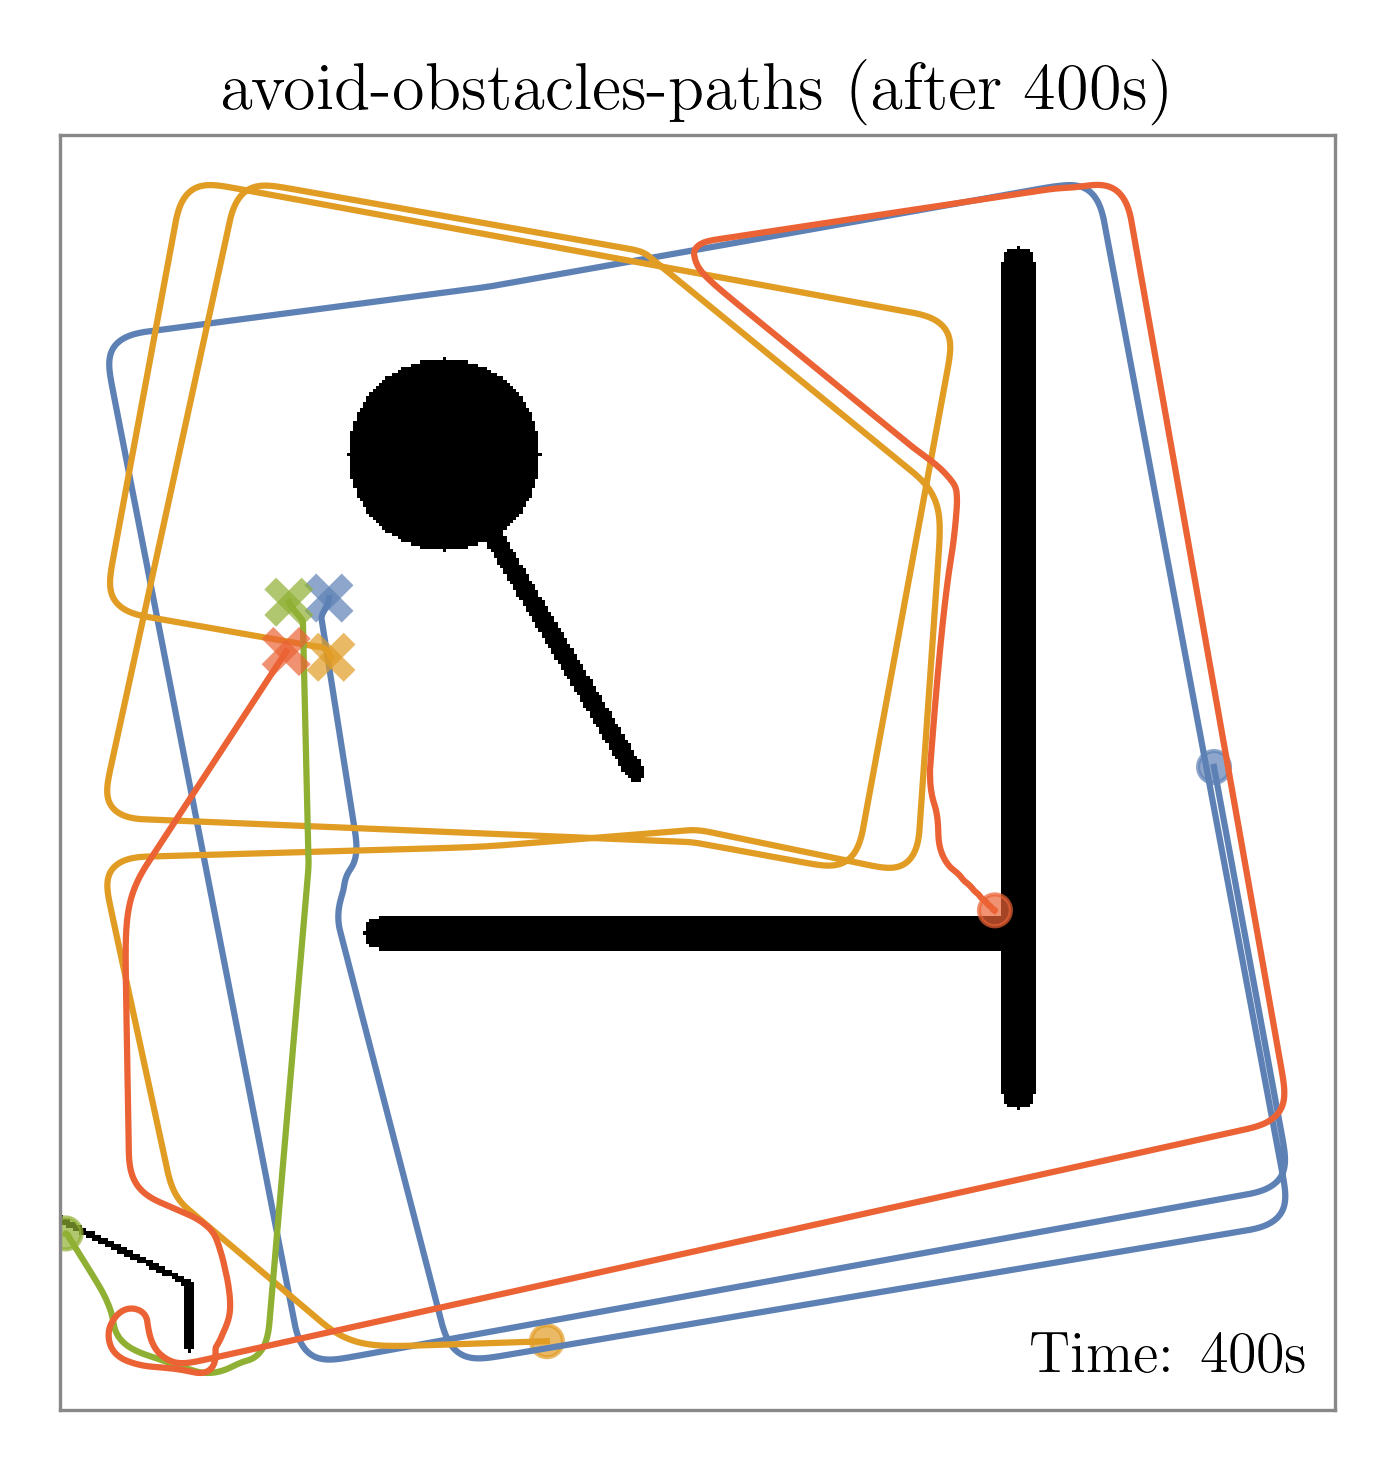
\includegraphics[width=\textwidth]{./figures/plots/paths/avoid-obstacles-paths-(after-400s).png}
    \end{subfigure}
    \begin{subfigure}[b]{\w}
        \centering
        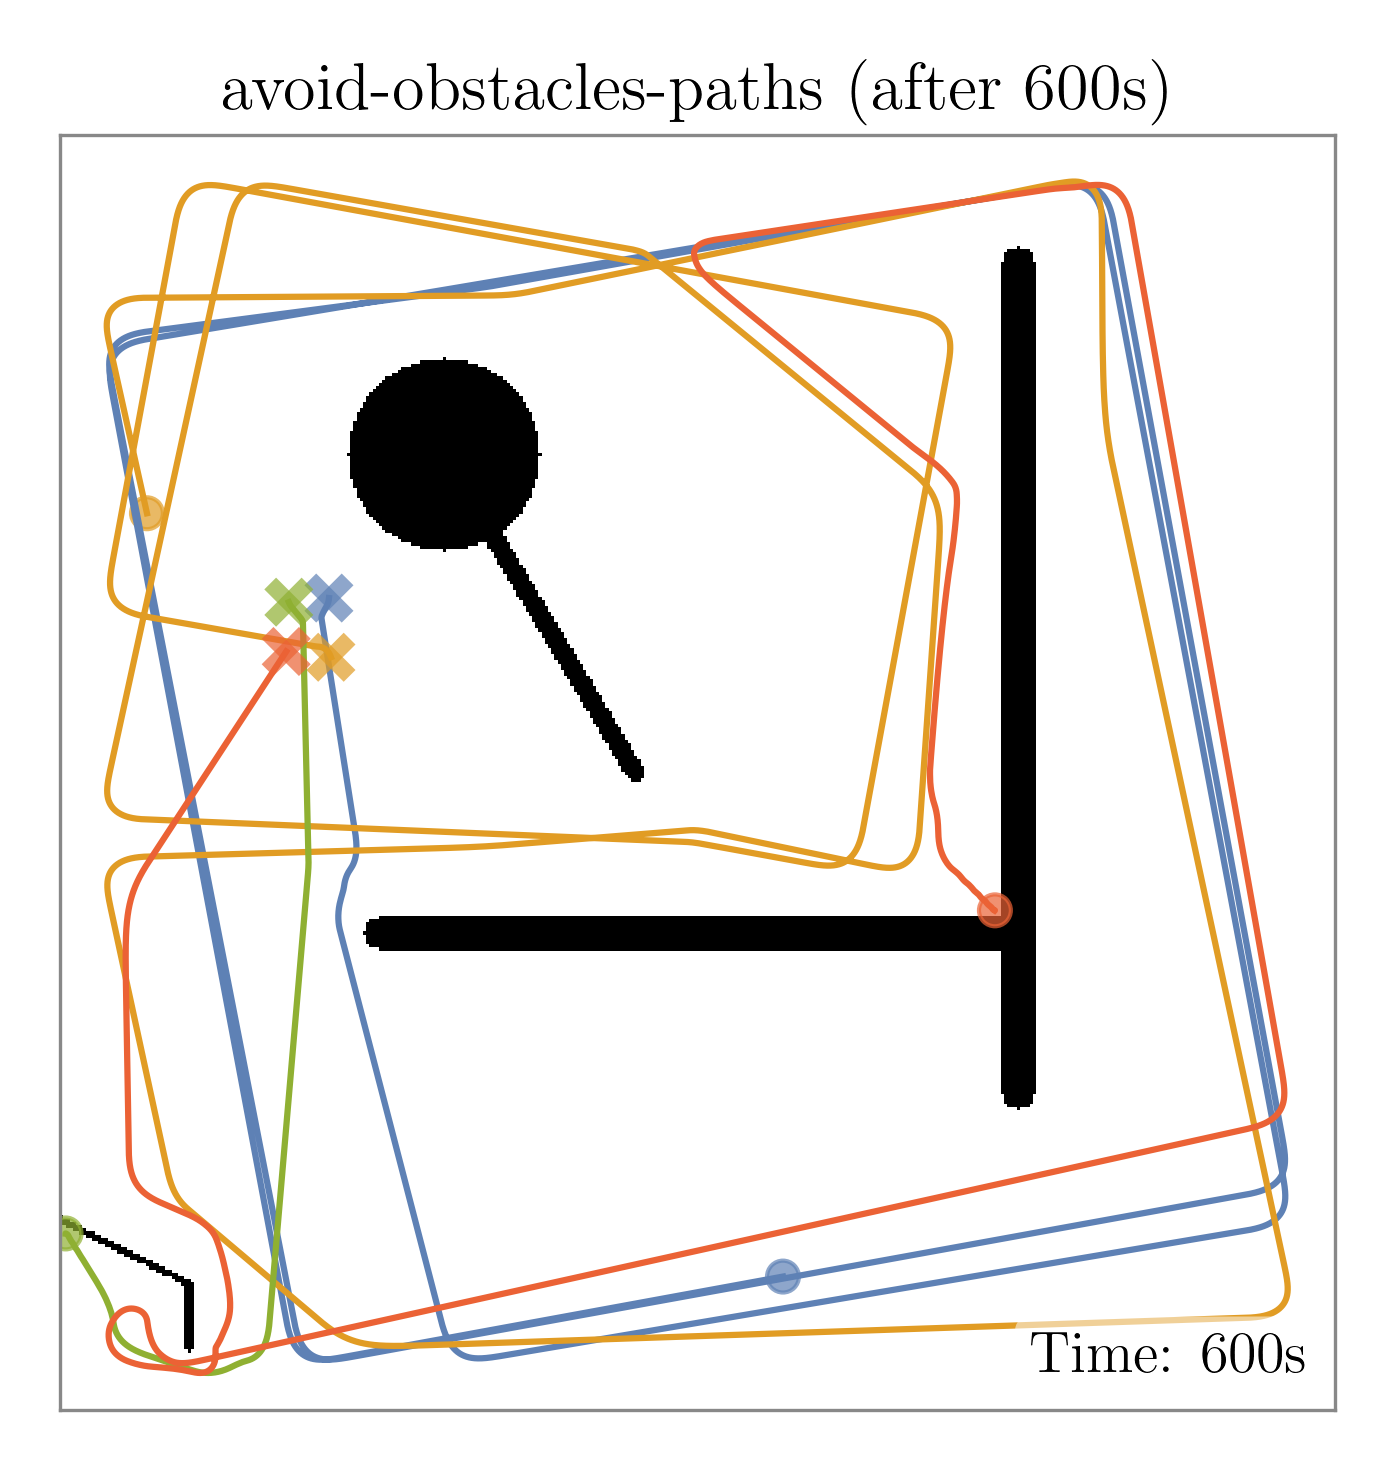
\includegraphics[width=\textwidth]{./figures/plots/paths/avoid-obstacles-paths-(after-600s).png}
    \end{subfigure}
    \caption{Paths of four robots running the Roomba algorithm at 200 s, 400 s, and 600 s in an example world simulated using \texttt{simple\_sim}. Crosses mark starting positions, and circles end positions.}
    \label{fig:roomba-paths}
\end{figure}

\subsection{Target Contributions}
Each robot maintains an internal state, which --- combined with sensor input --- drives its movement and exploration behavior. Conflicting objectives may arise; for instance, the robot may detect an unexplored area ahead, but find its path blocked by an obstacle. To resolve this, each behavior subsystem outputs a vector, a "target contribution", indicating its preferred movement. These vectors are summed to produce a single target vector, which dictates the robot’s final motion. Subsystems can be weighted according to their importance, obstacle avoidance, for instance, is typically given higher priority.

\subsection{Search Gradient}
\label{sec:search-gradient}

Each robot maintains a "search grid," which acts as a heatmap representing the exploredness of each cell in the map. This grid is continuously updated using the robot’s own observations and messages received from other robots via the shared communication channel. Explored areas are considered "cold," while unexplored areas and search objects are "hot".  \\

Assuming lossless communication, the search grids across robots should remain synchronized. Each robot computes a directional gradient from the search grid at its current position, encouraging movement toward hotter (less explored) regions. 

In practice, computing the gradient involves several steps. First, the average heat under the robot ($H$) must be calculated, using the cells underneath the robot ($C_H$), as in \cref{eq:robot-heat}. $N$ is the number of cells in $C_H$.

\begin{equation}
\label{eq:robot-heat}
    H = \frac{1}{N} \sum_{\;c\,\in\,C_H} \mathrm{heat}(c)
\end{equation}

Next, a vector $\mathbf{d}$ is computed from the robot's position $P$ to every grid cell ($C_\nabla$) within a specified radius $r$:

\begin{equation}
    \mathbf{d} = \mathrm{pos}(c) - P, \quad \forall c \in C_\nabla
\end{equation}

Each cell contribution to the final gradient, is based on the difference in heat between the cell and the heat under the robot, and its proximity to the robot in the direction of $\mathbf{d}$. The contribution fades linearly with distance, resulting in the following expression:

\begin{equation}
    \nabla = \sum_{c\,\in\,C_\nabla} \;
    \underbracket{\; \mathbf{d}/\norm{\mathbf{d}}      \;}_\text{\makebox[0pt]{Direction}} \cdot
    \underbracket{\; \big(\mathrm{heat}(c) - H\big)    \;}_\text{Heat Difference} \cdot
    \underbracket{\; \big(1 - \norm{\mathbf{d}}/r\big) \;}_\text{Nearness}
    \label{eq:fade-gradient}
\end{equation}

This formulation works well in open areas but may behave undesirably near map edges. Since cells outside the map have no heat value and negative contributions repel the robot, the gradient can incorrectly point toward the map boundary if surrounding cells inside the map are colder than the robot position.  \\

To address this, only positive heat differences are considered in the gradient calculation. In practice, this means that the gradient points towards the "hottest" direction, but not necessarily away from the "coldest" direction.

\begin{equation}
\label{eq:robot-gradient}
    \nabla = \sum_{c\,\in\,C_\nabla}
    \begin{cases}
        \mathbf{d}/\norm{\mathbf{d}}      \; \cdot
        \big(\mathrm{heat}(c) - H\big)    \; \cdot
        \big(1 - \norm{\mathbf{d}}/r\big) \; \quad &\text{if } \mathrm{heat}(c) > H
        \\
        0, \quad &\text{otherwise}
    \end{cases}
\end{equation}

This modification prevents attraction toward map boundaries and ensures the robot continues to seek out unexplored areas. Cells occluded by obstacles are also excluded from the gradient computation.


\subsection{Proximity Grid}
To maintain simulated network connectivity, robots must stay within communication range of each other. Each robot uses a "proximity grid" to estimate which areas of the map are within range of the main robot network.

\begin{figure}[H]
    \begin{center}
        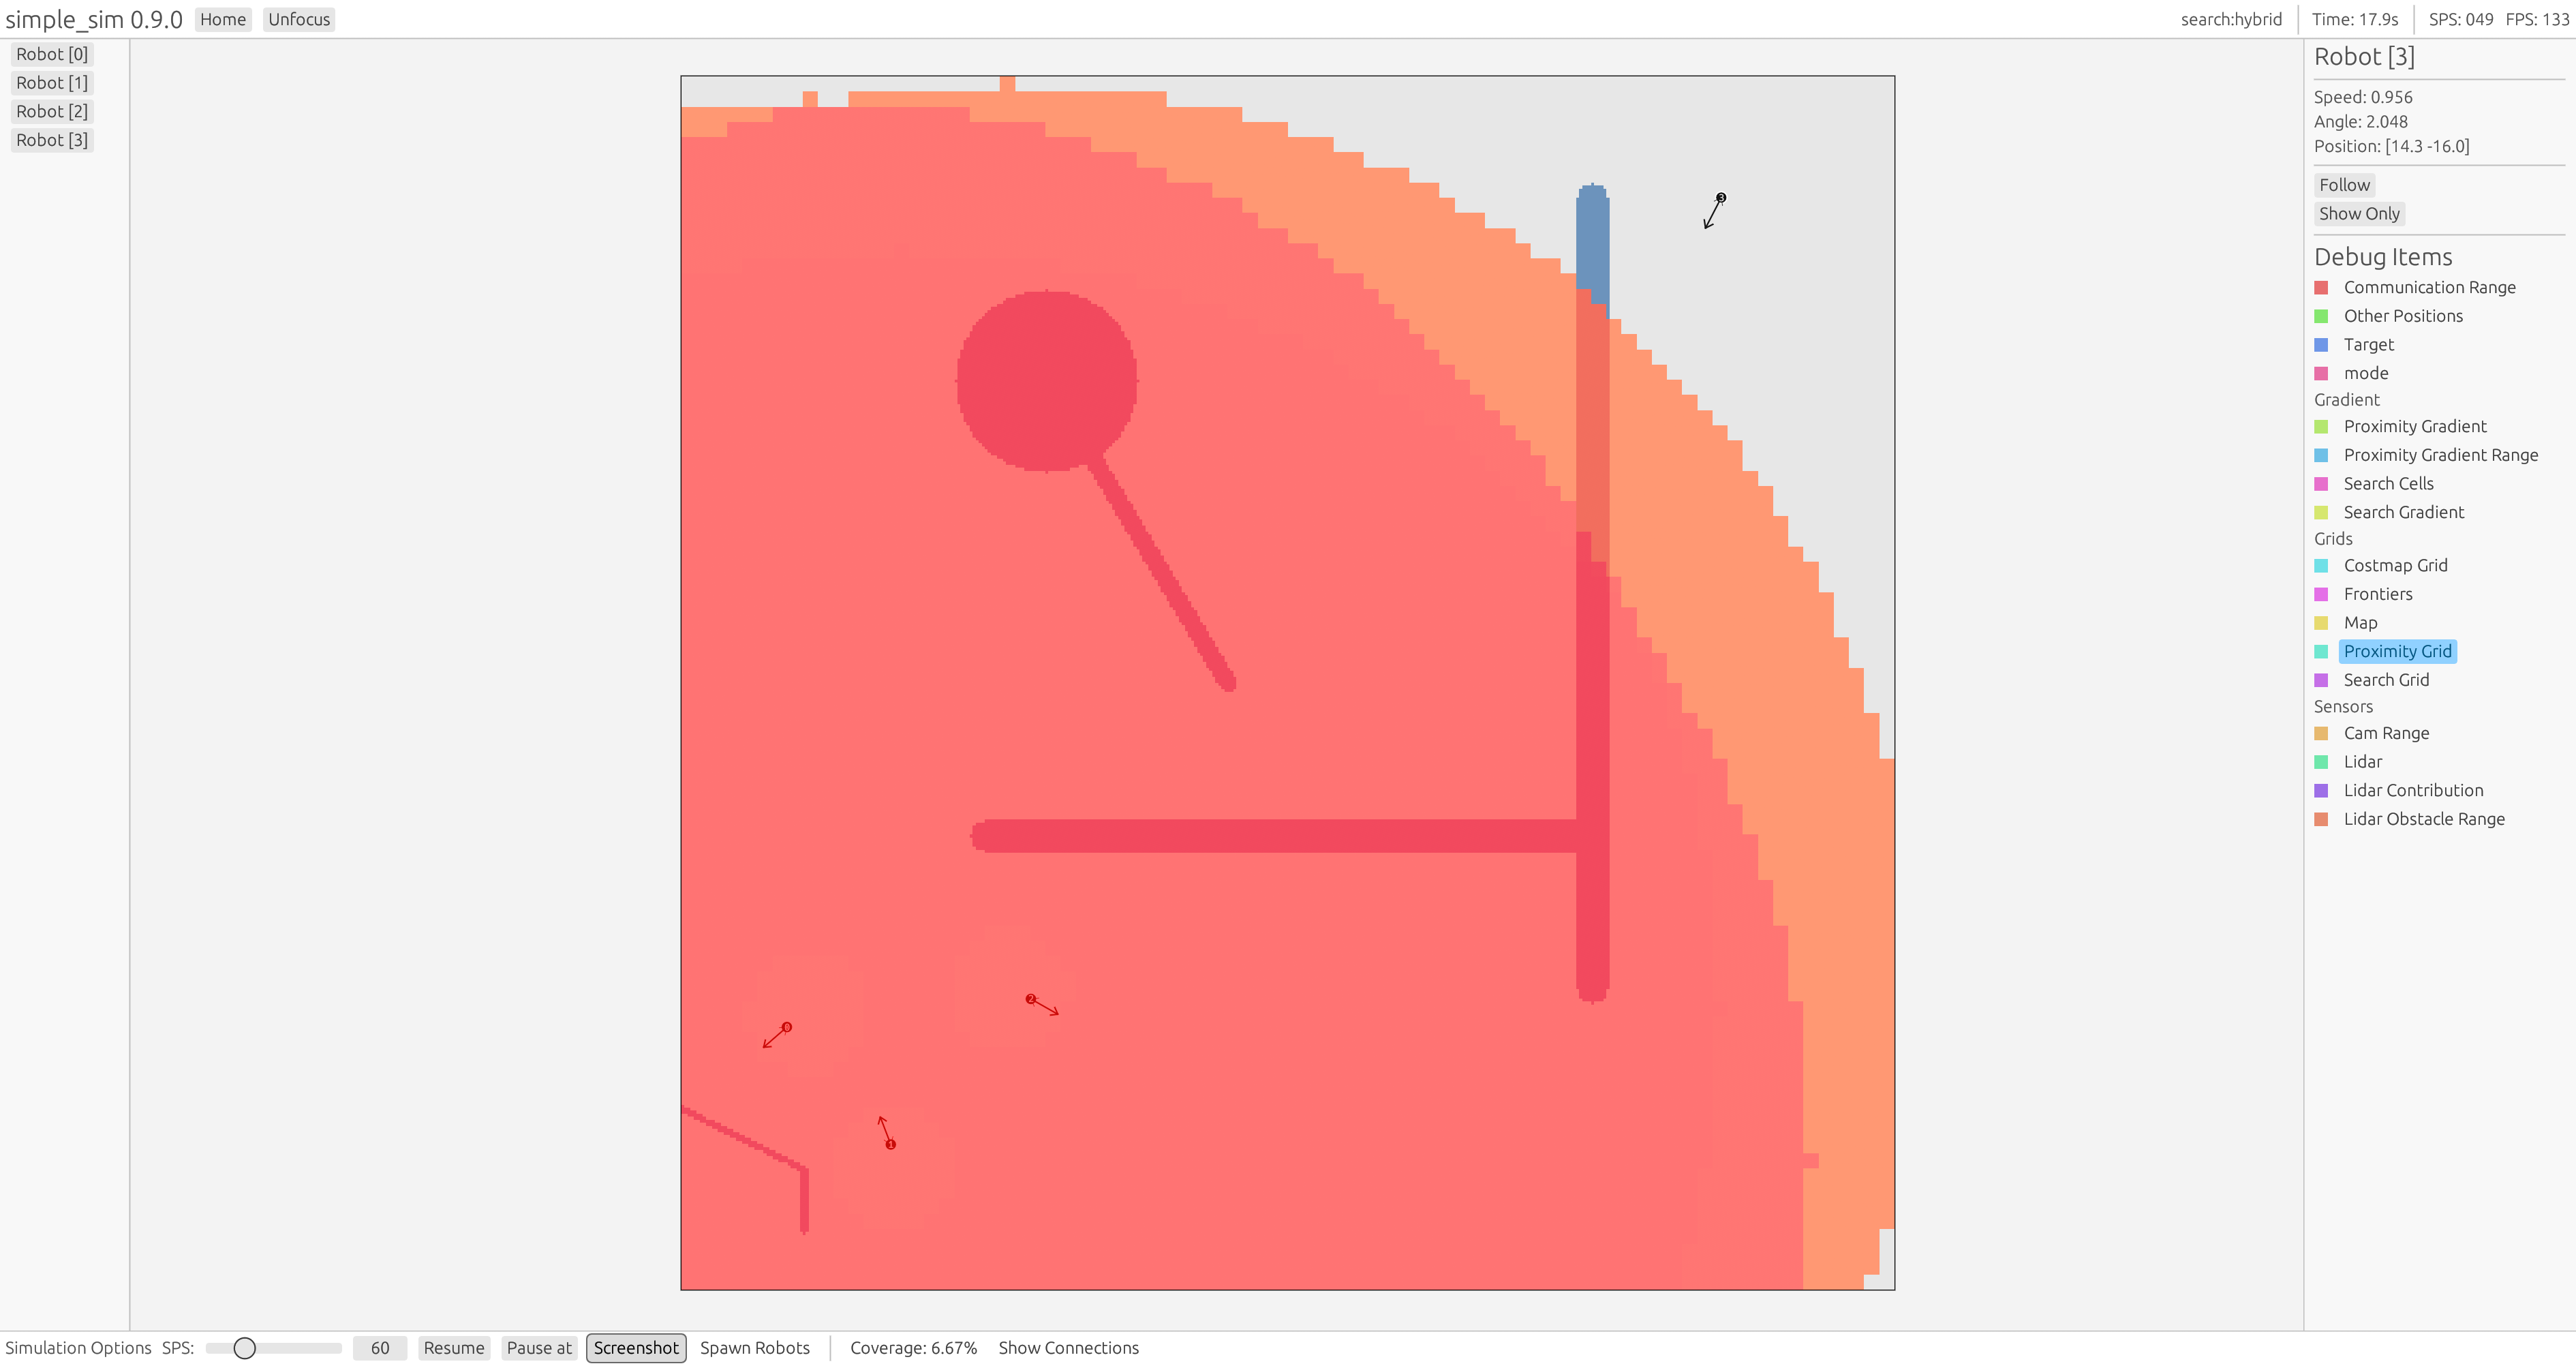
\includegraphics[width=0.45\textwidth]{figures/screenshots/proximity-gradient.png}
    \end{center}
    \caption{Proximity grid showing 3 robots forming the main network and a disconnected robot is heading towards the main network.}
    \label{fig:proximity-grid}
\end{figure}

The proximity grid is computed by identifying the largest set of connected robots and "coloring" their communication range. Tiles connected by a single robot are half-shaded to indicate weaker signal reliability (see \cref{fig:proximity-grid}). A gradient is computed over this grid and added as a weighted contribution to the robot’s overall target vector. \\

Importantly, each robot excludes itself when calculating the proximity grid. This ensures that if a robot is the sole link between two clusters, it will move toward the main network and draw disconnected robots with it.

\subsection{Gradient Based-Algorithm}
The gradient-based algorithm calculates the robot's "target" vector using contributions from both the search and proximity grid gradients. However, when relying solely on these contributions, the resulting target vector often points sideways or even backward. This occurs because the robot continuously "cools" down the area in camera's field of view, which leads to excessive turning and minimal forward progress. \\

To mitigate this, a small constant forward vector is added to the total target vector to maintain movement and promote map coverage. \Cref{fig:gradient-paths} illustrates the paths of four robots executing this behavior.

\def\w{0.329\textwidth}
\begin{figure}[H]
    \centering
    \begin{subfigure}[b]{\w}
        \centering
        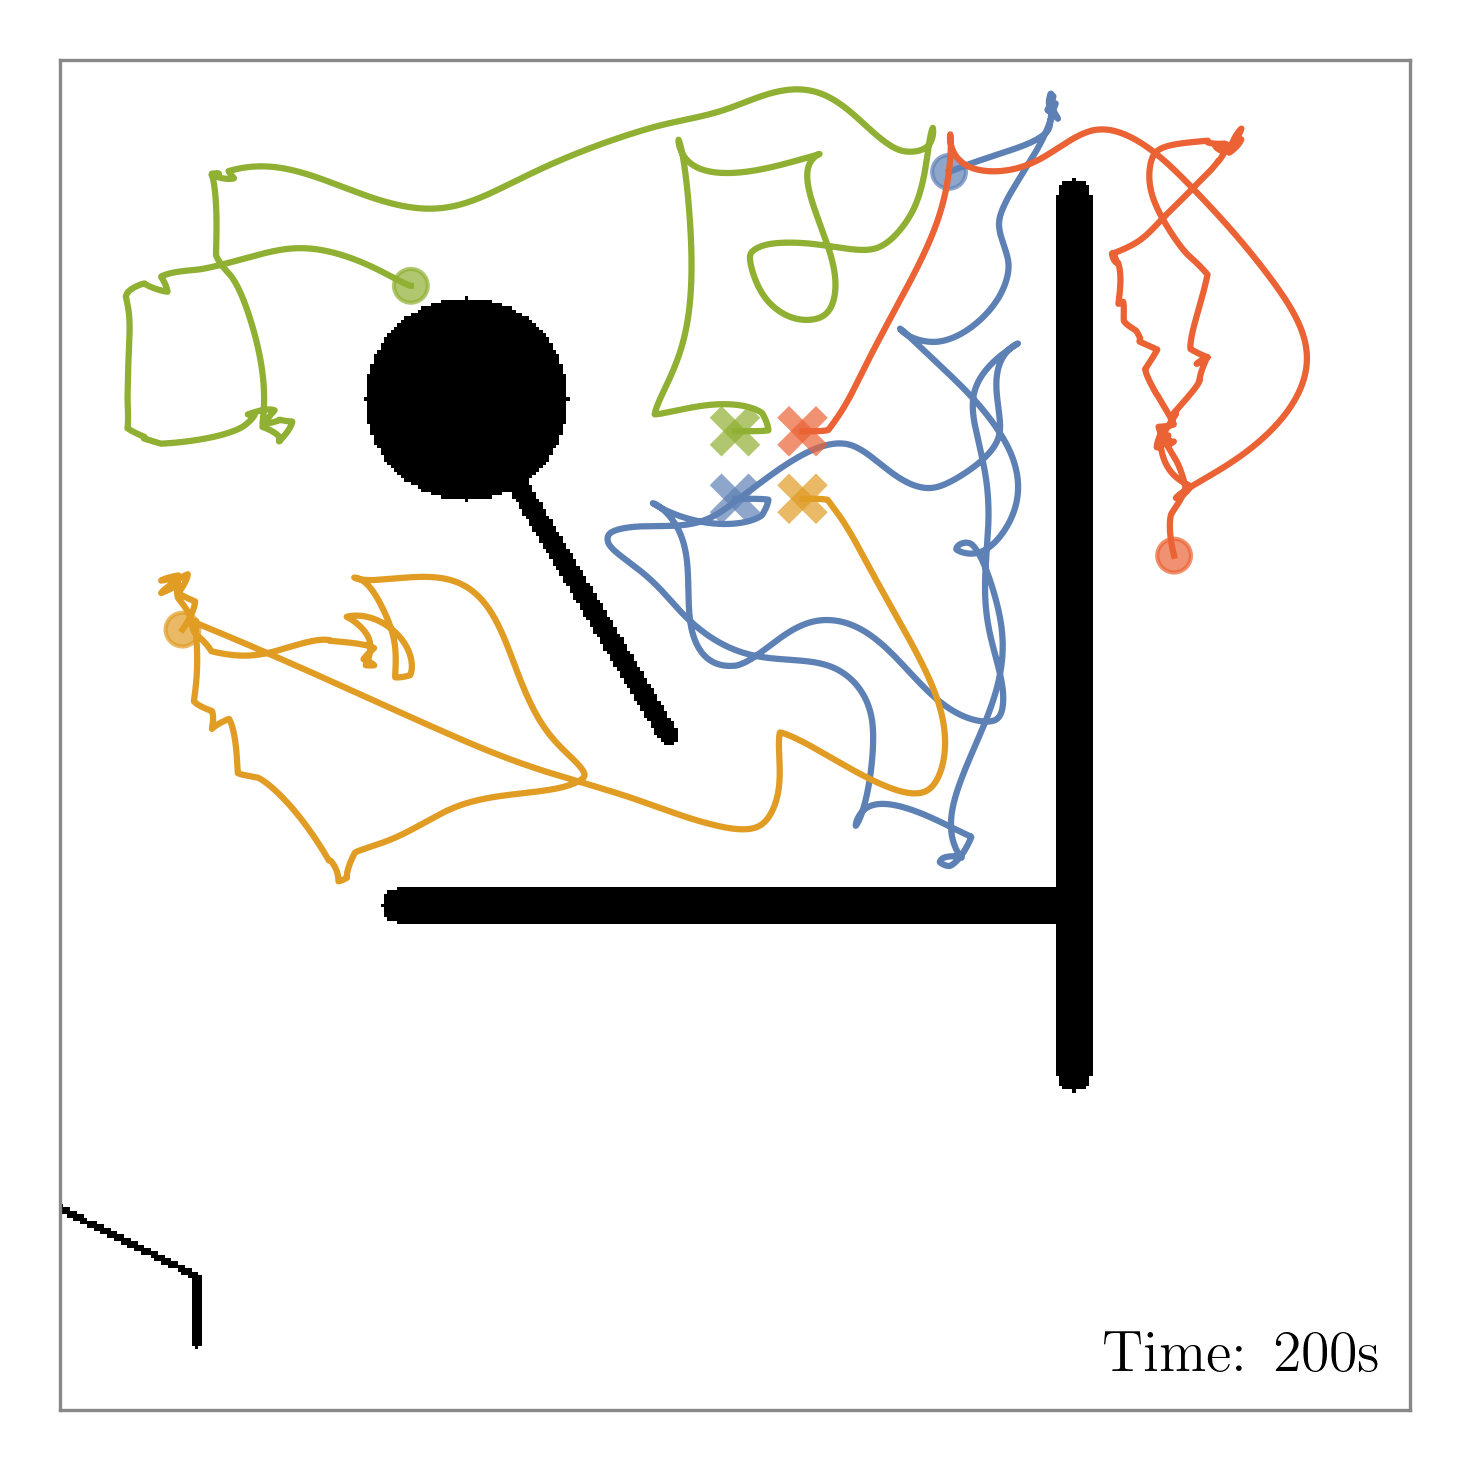
\includegraphics[width=\textwidth]{./figures/plots/paths/search:gradient-paths-(after-200s).png}
    \end{subfigure}
    \begin{subfigure}[b]{\w}
        \centering
        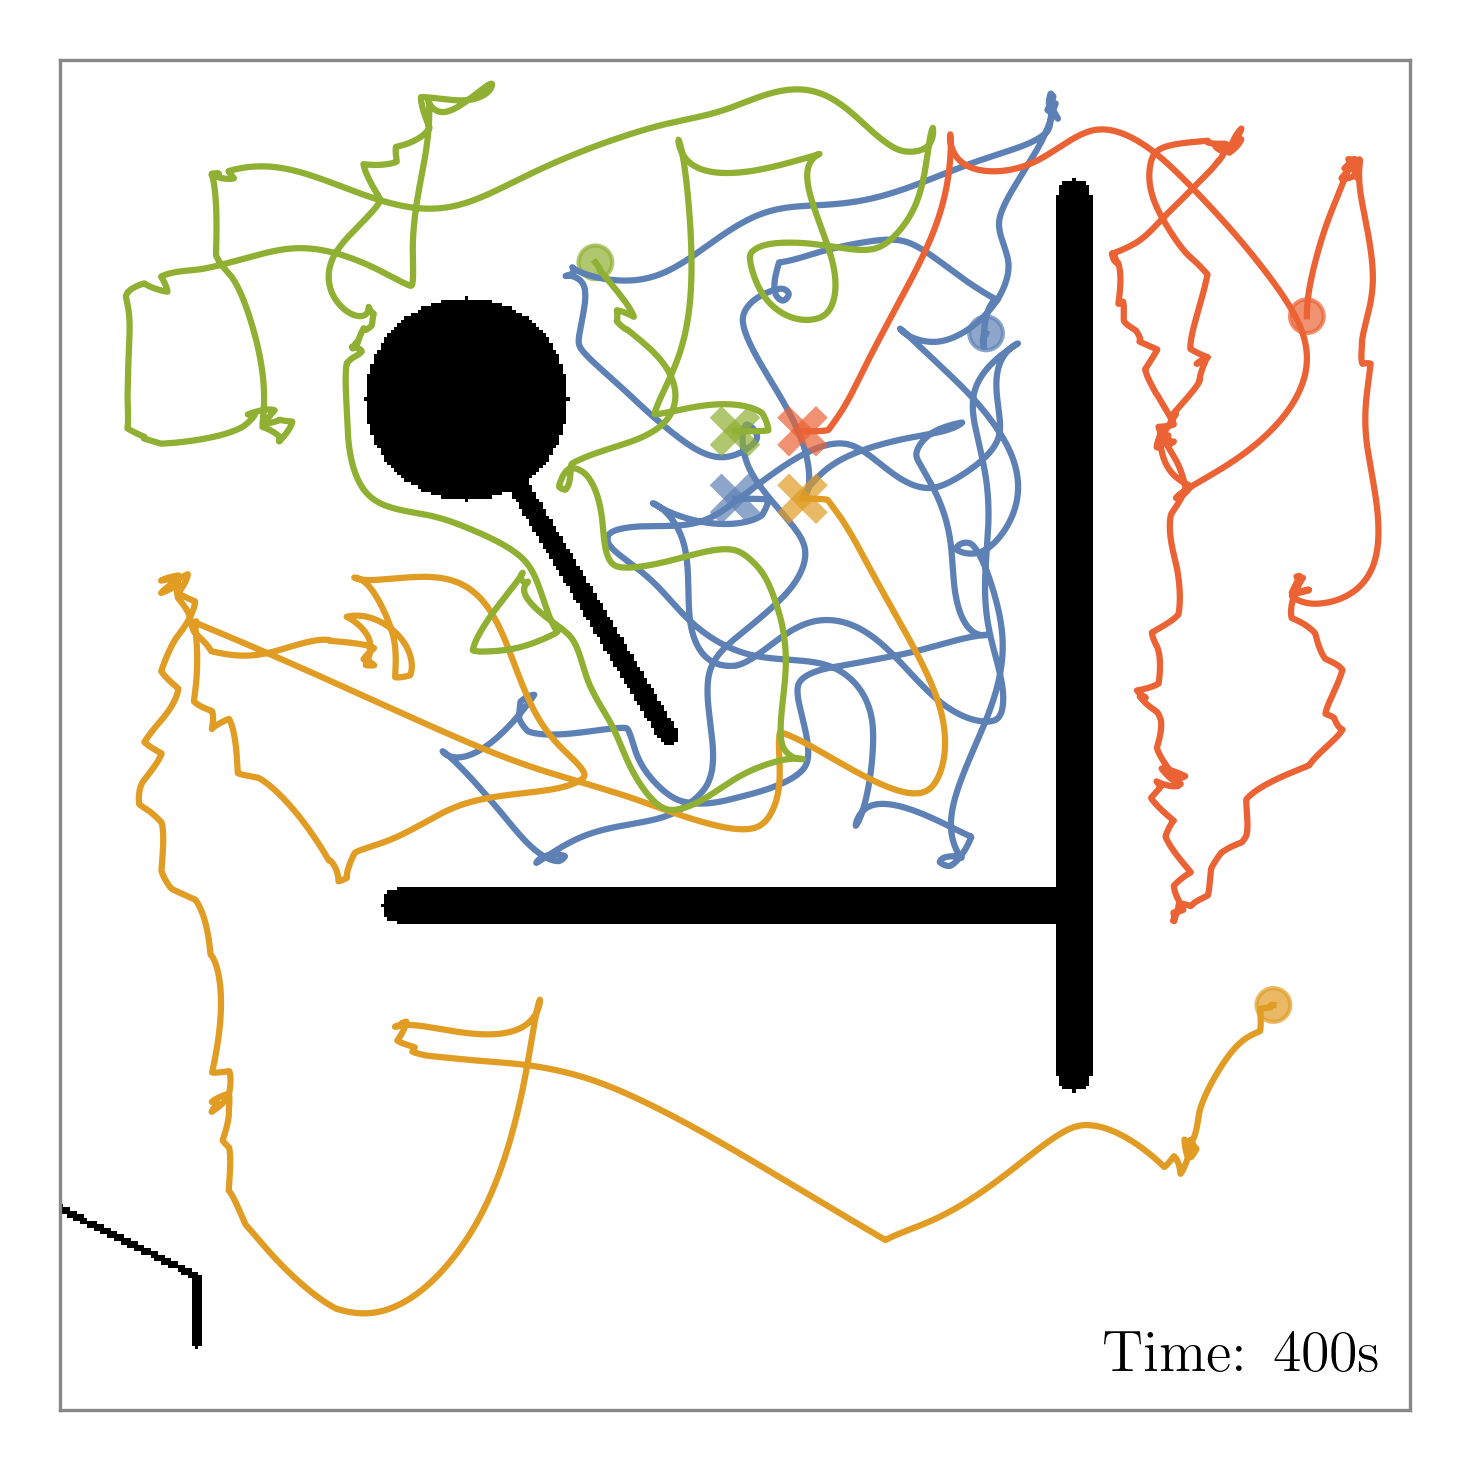
\includegraphics[width=\textwidth]{./figures/plots/paths/search:gradient-paths-(after-400s).png}
    \end{subfigure}
    \begin{subfigure}[b]{\w}
        \centering
        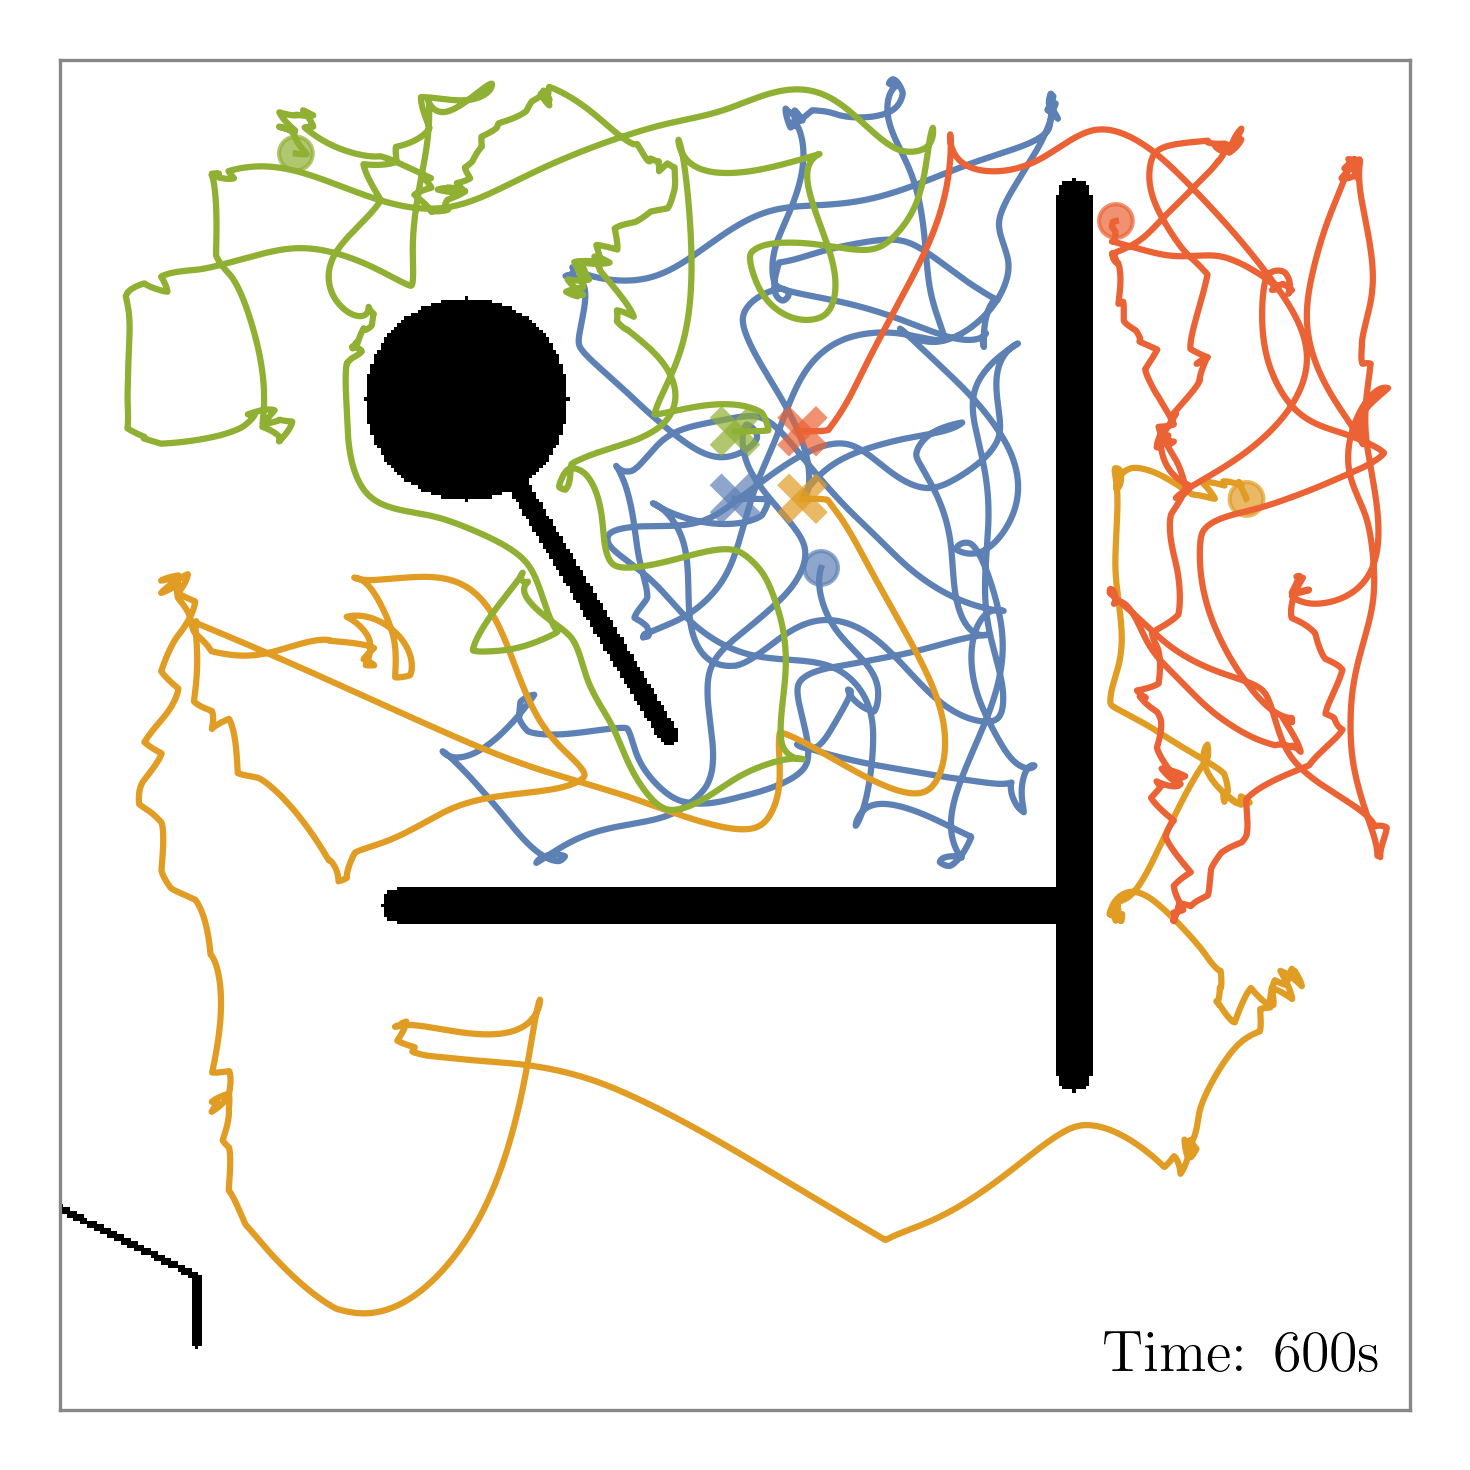
\includegraphics[width=\textwidth]{./figures/plots/paths/search:gradient-paths-(after-600s).png}
    \end{subfigure}
    \caption{Paths of four robots running the gradient-based algorithm at 200 s, 400 s, and 600 s in an example
    world simulated using \texttt{simple\_sim}. Crosses mark starting positions, and circles end positions.}
    \label{fig:gradient-paths}
\end{figure}

The robots explore the environment effectively but tend to linger in already explored regions. This behavior may be due to the limited range of the search gradient. Additionally, robots exhibit more erratic paths when the gradient magnitude becomes small. In general, robots switch between smooth trajectories in unexplored areas and jagged paths when trapped in previously covered regions. \\

In \cref{fig:gradient-forward-bias}, the search grid is visualized. Here the robots are moving towards unexplored or hotter areas.
\begin{figure}[H]
  \centering
  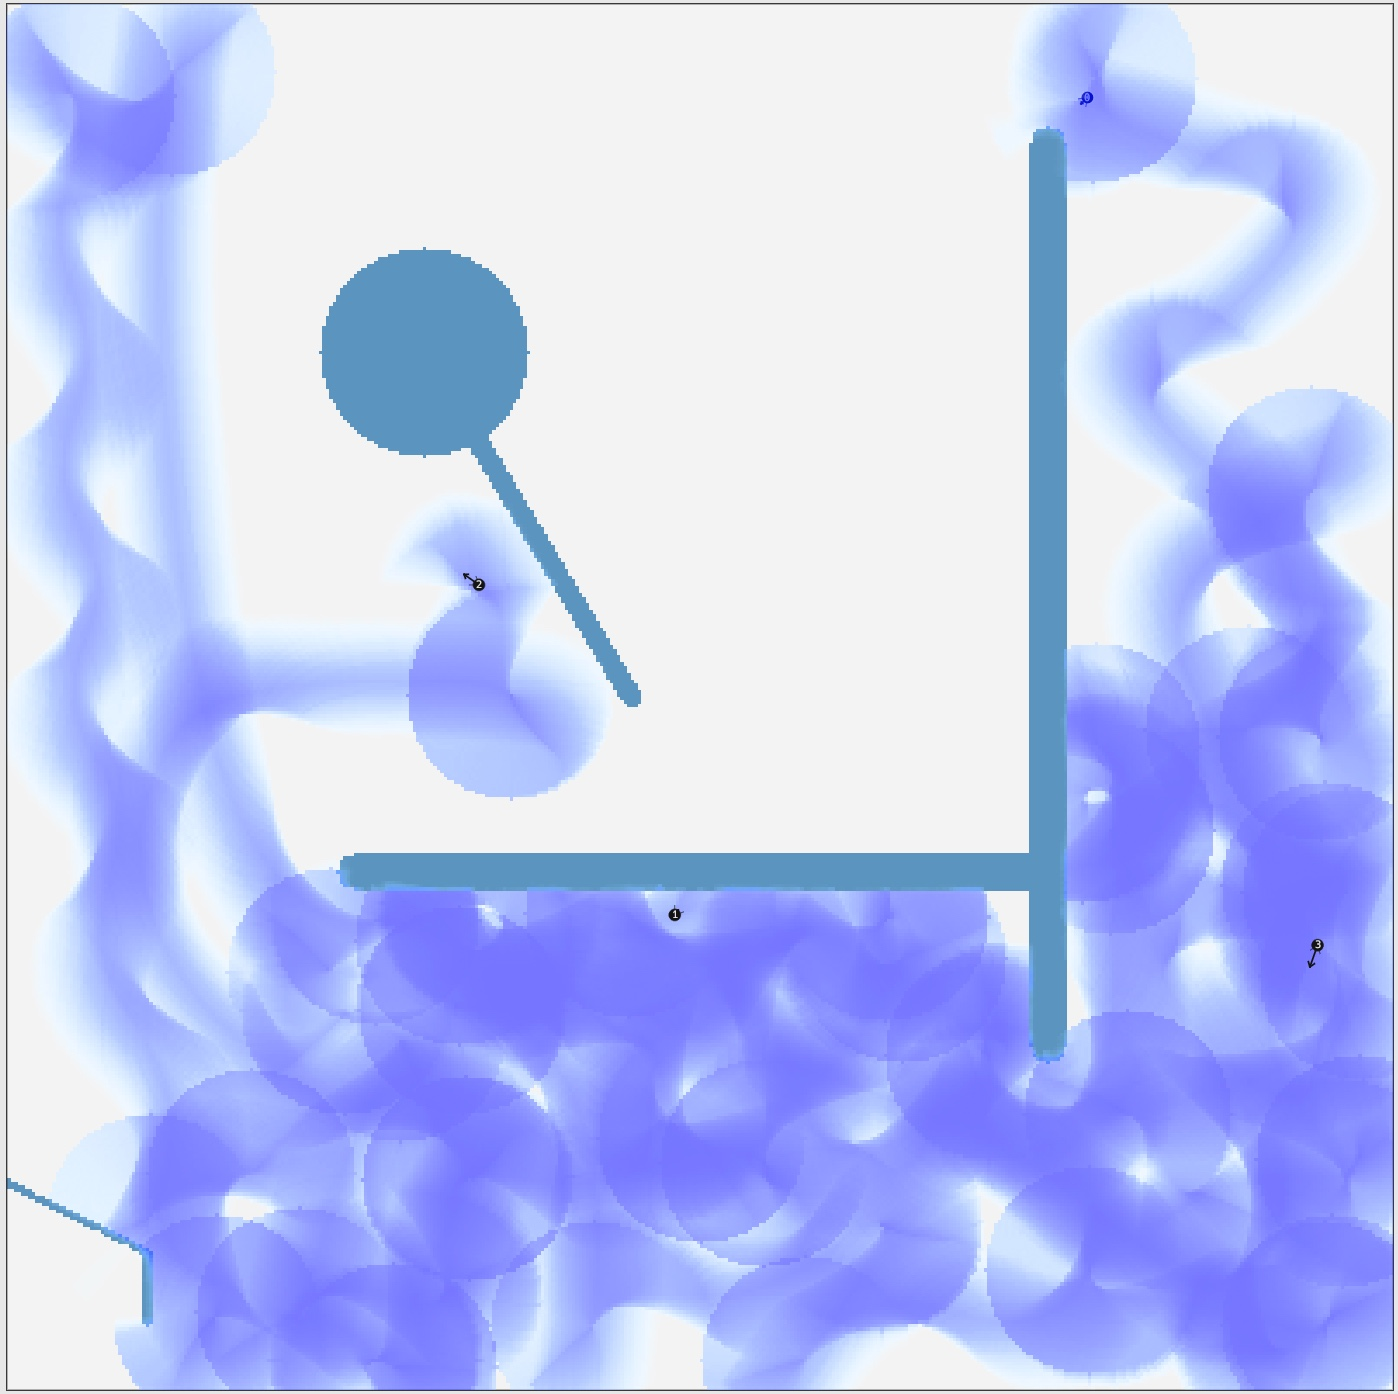
\includegraphics[width=0.45\textwidth]{./figures/screenshots/with-forward.jpeg}
  \caption{The search grid, where darker blue shows the cooler aeras..}
  \label{fig:gradient-forward-bias}
\end{figure}

To improve coverage, mechanisms that encourage movement toward globally unexplored areas would be beneficial.

\subsection{Global Planner}
When the search gradient fails to provide a clear direction --- i.e., when the robot lacks a local preference --- a global planner is used to guide the robot to a more promising unexplored region. The global planner operates according to the following procedure:

\begin{enumerate}
  \item Generate a costmap (\cref{sec:costmap}).
  \item Identify frontiers and group them into regions \cite{frontier-exploration} (\cref{sec:frontier_exploration}).
  \item Evaluate the frontiers and select a goal (\cref{sec:frontier_exploration}).
  \item Plan a path using a straight line or the A* algorithm \cite{a-star} (\cref{sec:path_planning}).
  \item Follow the path until the goal is reached or the path is invalidated (\cref{sec:path_following}).
\end{enumerate}
 
\subsubsection{Costmap}
\label{sec:costmap}
The costmap is a grid-based representation of the environment with a variable resolution. Each cell in the costmap is assigned one of three states:

\begin{itemize}
  \item \textbf{Searched:} Cells identified as covered in the search grid.
  \item \textbf{Unknown:} Cells not yet visited.
  \item \textbf{Obstacle:} Cells corresponding to known obstacles or other robots, inferred from recent LiDAR readings.
\end{itemize}

The costmap is used in both frontier exploration and path planning. To ensure safe navigation, the robot must avoid collisions with obstacles as well as other robots. Therefore, when evaluating potential paths or frontiers, the surrounding cells are also checked to ensure they are free of obstacles. The number of surrounding cells considered depends on a configurable clearance parameter, which defines the minimum required buffer between the robot and nearby obstacles. \\

This clearance can be dynamically adjusted over time --- for example, allowing the robot to take riskier, narrower paths during later stages of the search when unexplored areas become harder to reach. This adaptive behavior helps maintain efficiency without compromising early-stage safety.

An example of the costmap and its affect on path planning is shown in \cref{fig:path_planning} on page \pageref{fig:path_planning}.


\subsubsection{Frontier Exploration}
\label{sec:frontier_exploration}
A frontier is defined as a boundary between explored and unexplored regions. These frontiers are discovered using a Breadth-First Search (BFS) starting from the robot's current position. This approach avoids a full costmap scan, thereby reducing computational overhead. \\

Detected frontier cells are grouped into regions and scored based on:

\begin{itemize}
  \item Frontier region size
  \item Distance to the robot
  \item Required turn angle to face the frontier
\end{itemize}

As mentioned, frontiers must meet a minimum obstacle clearance threshold to be considered valid as a potential goal.\\

An experiment was conducted in two environments to evaluate the coverage performance with a range of different weights, see \cref{fig:frontier-eval-params}. 
All tested configurations will eventually achieved full map coverage; therefore, performance is evaluated based on coverage speed.
\begin{figure}[H]
    \centering
    \begin{subfigure}[b]{0.49\textwidth}
        \centering
        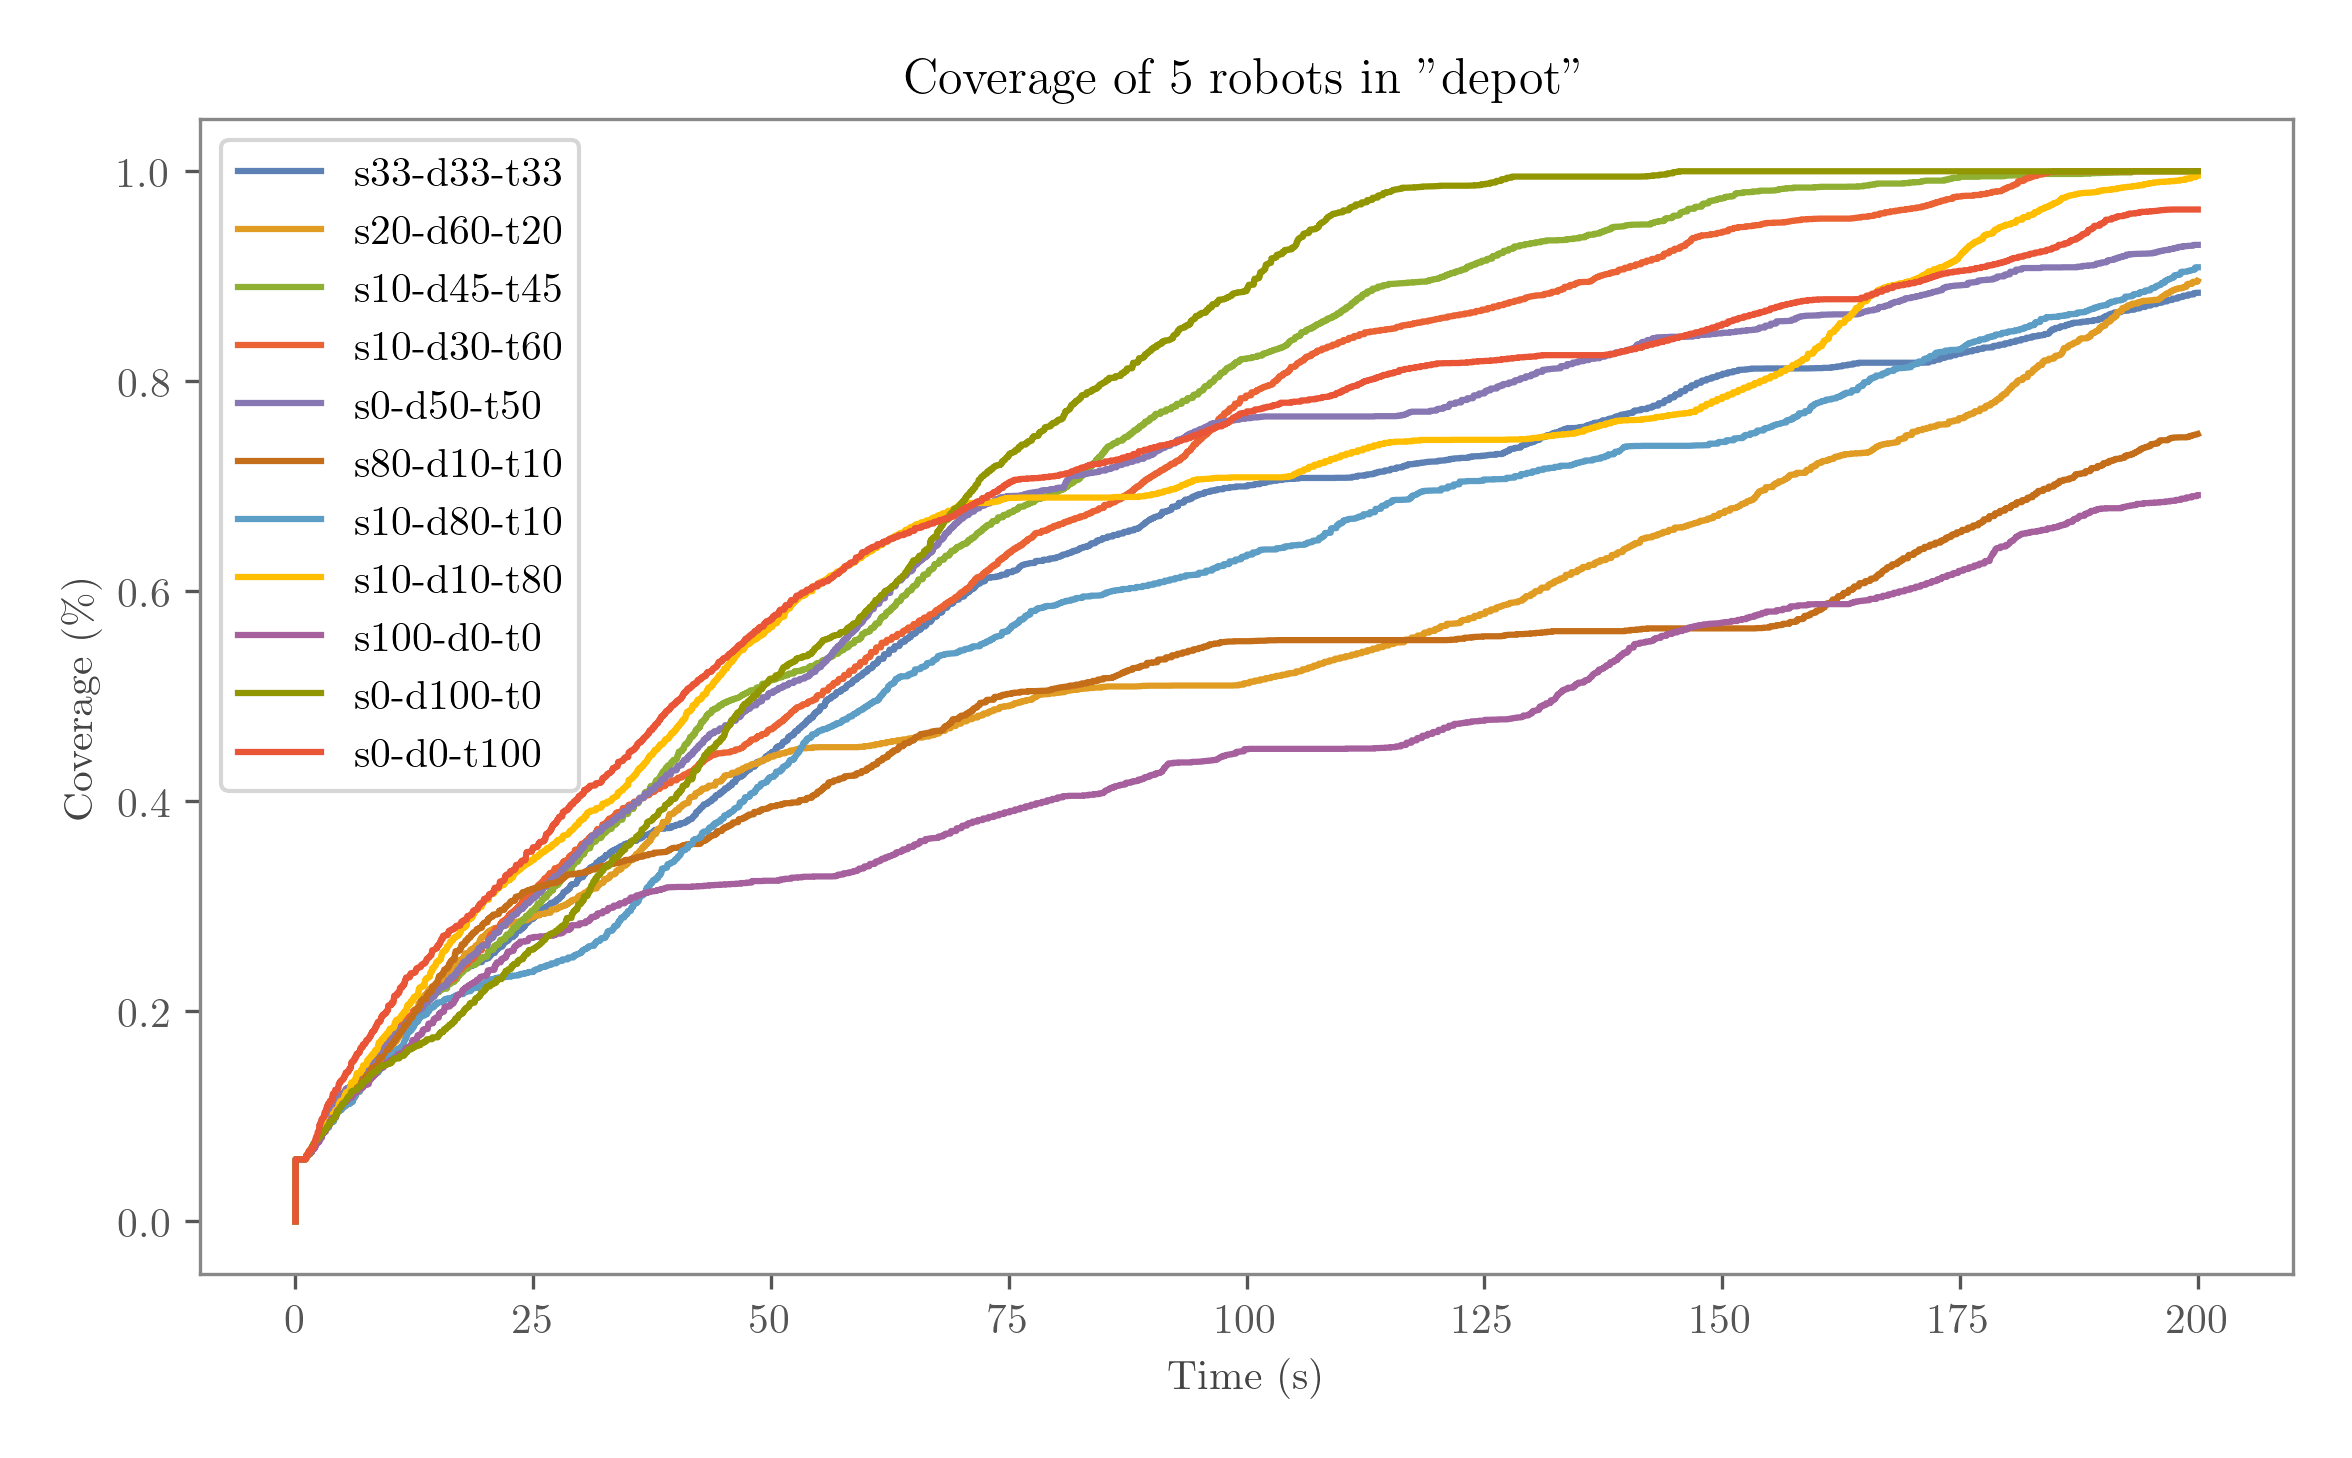
\includegraphics[width=\textwidth]{figures/frontier_eval_params_depot.png}
        \caption{Simple map}
    \end{subfigure}
    % \hfill
    \begin{subfigure}[b]{0.49\textwidth}
        \centering
        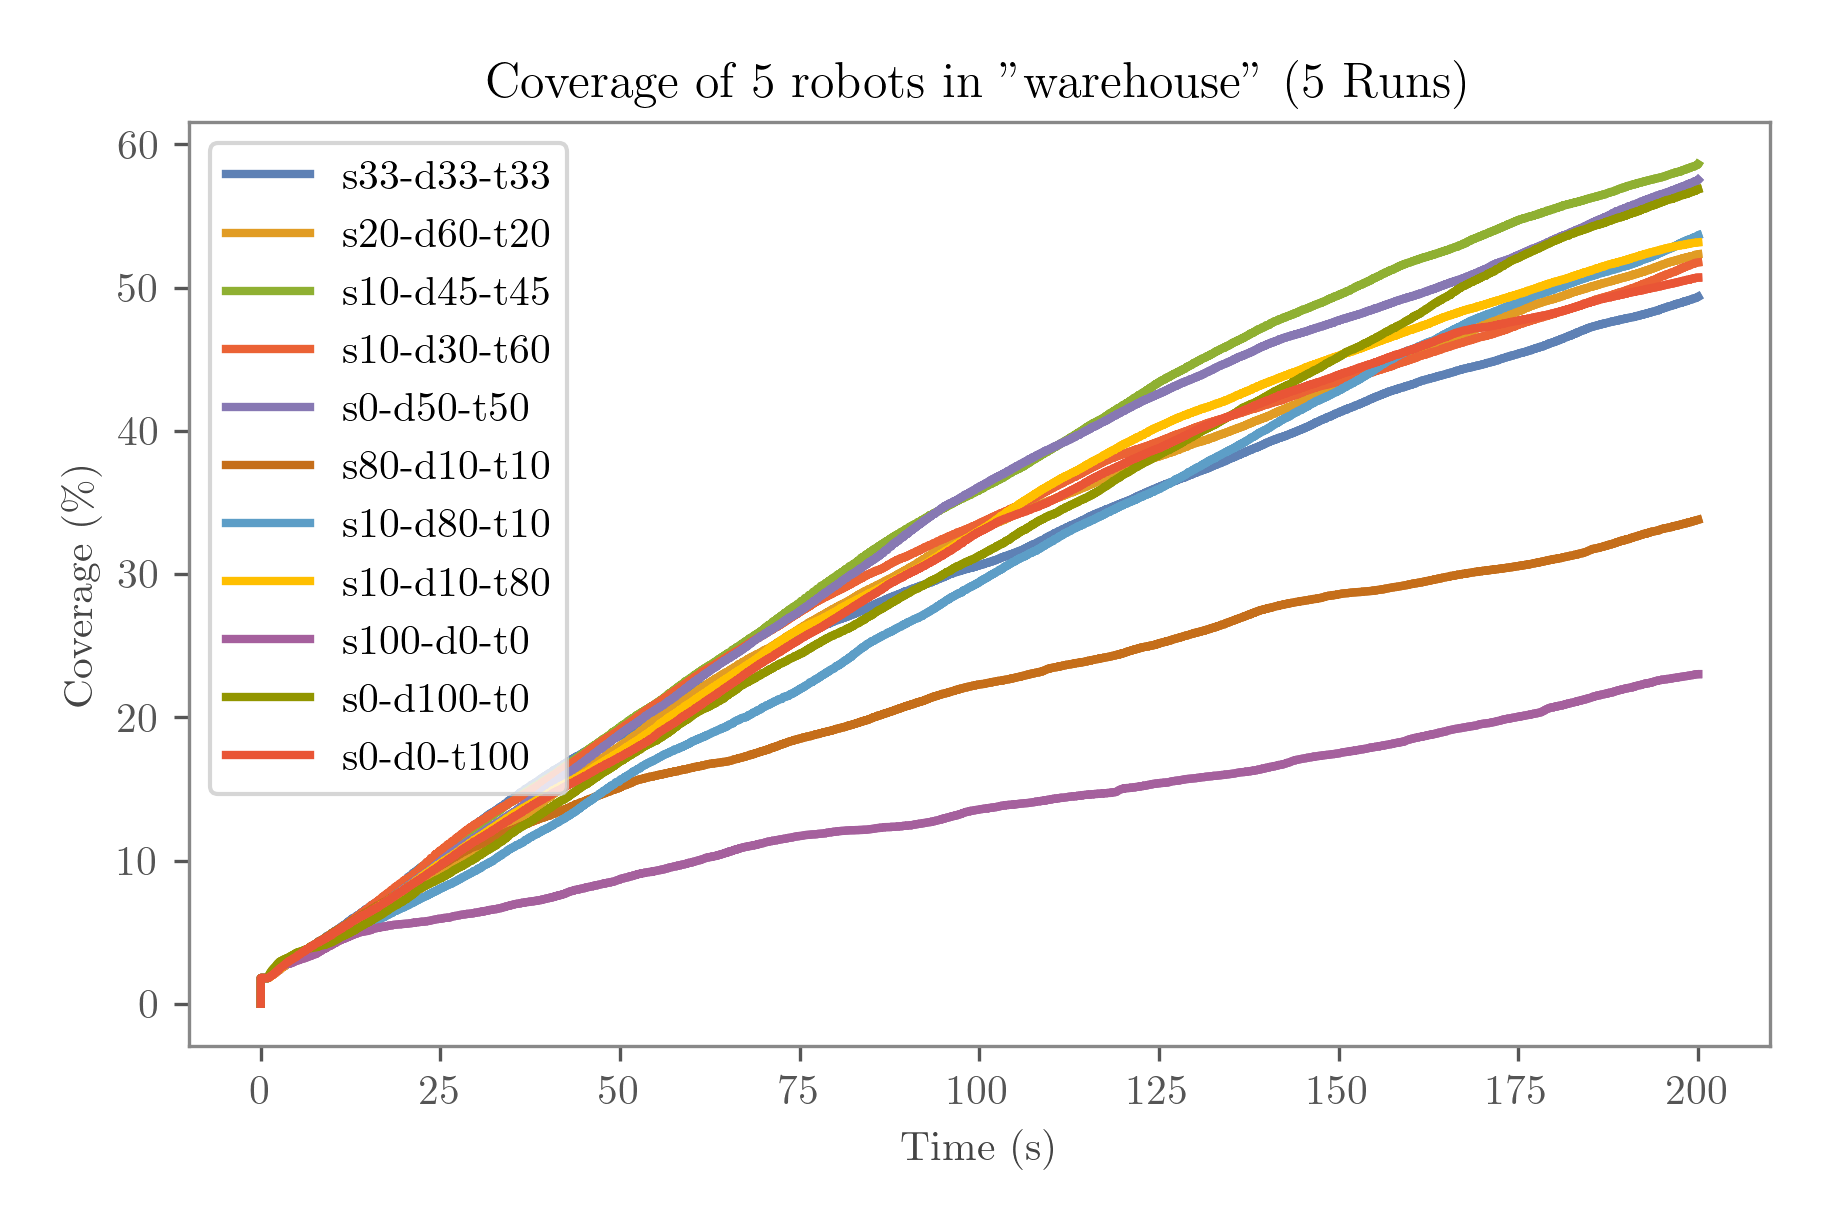
\includegraphics[width=\textwidth]{figures/frontier_eval_params_warehouse.png}
        \caption{Complex map}
    \end{subfigure}
    \caption{Frontier evaluation parameters comparison. The weights are: \texttt{sXX} for frontier size, \texttt{dXX} for distance to the frontier, and \texttt{tXX} for the required turn angle.}
    \label{fig:frontier-eval-params}
\end{figure}

Configurations that prioritized distance and turn angle produced the fastest coverage. This outcome suggests that minimizing rotation allows for higher sustained forward velocity. In contrast, configurations that emphasized frontier size alone often resulted in inefficient behavior, such as long detours and frequent turning, which slowed down overall progress. The final parameter configuration, \texttt{s10-d45-t45}, produced the overall best and most consistent performance across maps with various complexity.

\subsubsection{Path Planning}
\label{sec:path_planning}
Once a goal is selected, the planner first attempts to generate a direct, straight-line path to the goal. If this path violates the required clearance from obstacles or other robots, the planner falls back to the A* algorithm.\\

The A* algorithm explores the grid by combining the cumulative path cost with a heuristic estimate of the remaining distance to the goal. A min-heap (priority queue) is used to efficiently select the next cell to expand based on the lowest estimated total cost. Only collision-free cells that satisfy the clearance constraint are considered during expansion.\\

Once the goal is reached, the resulting path consists of the sequence of cells from the start to the goal. This path is then post-processed to remove unnecessary intermediate points, provided that the smoothed path still maintains the required clearance. This smoothing step reduces path length and ensures more natural robot motion while preserving safety.

\begin{figure}[H]
  \begin{center}
    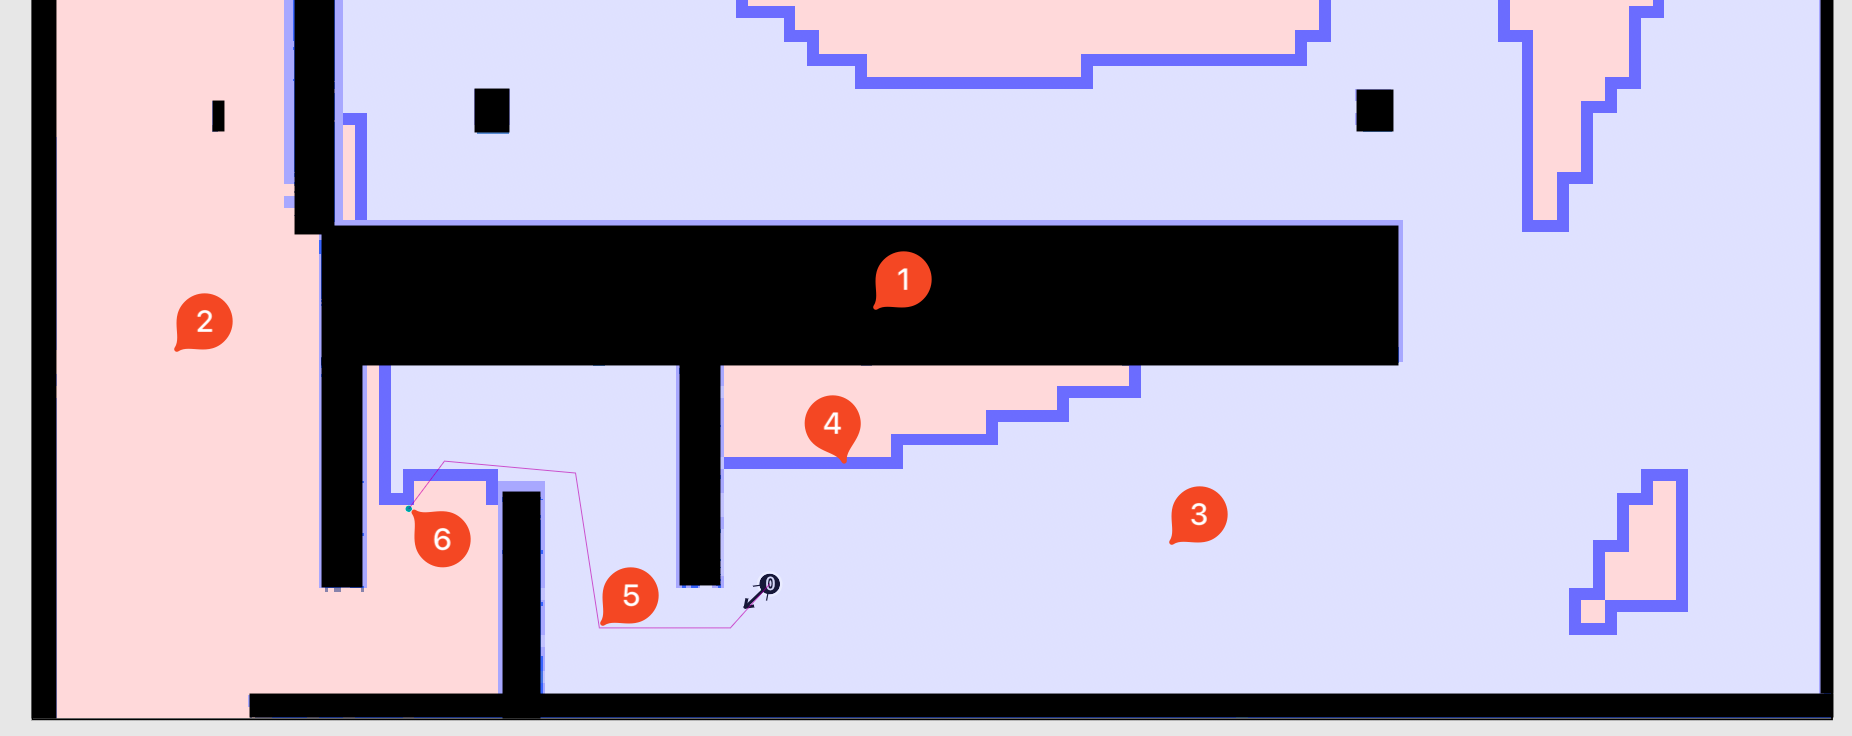
\includegraphics[width=0.95\textwidth]{./figures/screenshots/path-planning-edit.png}
  \end{center}
  \caption{Screenshot of global path planner components in \texttt{simple\_sim}: 1) obstacle cells, 2) unexplored cells, 3) explored cells, 4) frontier cells, 5) goal path, and 6) goal.}
  \label{fig:path_planning}
\end{figure}


\subsubsection{Path Following}
\label{sec:path_following}
The robot follows the planned path as a sequence of waypoints. As each waypoint is reached, it is marked as visited and removed from the remaining path. \\

To ensure robustness in dynamic environments, the path is continuously validated using the costmap. If the clearance to the next waypoint becomes invalid due to a newly detected obstacle, the robot does not immediately discard the path. Instead, it continues toward the waypoint, while incorporating reactive feedback from the LiDAR sensor. \\

LiDAR input takes precedence over the path-following command. For example, if a new obstacle appears directly in front of the robot, the repulsive contribution from the LiDAR cancels out the forward path-following command, causing the robot to stop. In less obstructed cases—such as when an obstacle appears on the front-right side—the robot will adjust its heading and veer left to navigate around it. \\

If the path fails clearance checks repeatedly, the planner attempts to replan a new path to the current goal. However, in some cases, no viable path may exist due to dynamic obstructions. In such scenarios, the robot will abandon the current goal and select a new one. \\

Additionally, if a robot becomes disconnected from the swarm, a new goal is generated to guide it back toward the network. This reconnection behavior uses the proximity grid to identify areas with higher robot density, helping to restore communication.

\subsection{Hybrid Algorithm}
The global planner enables a hybrid algorithm that combines both local and global strategies. As long as the local search gradient provides a sufficiently strong direction, the robot continues using the gradient-based method. When the gradient magnitude falls below a predefined threshold, the global planner is triggered to relocate the robot to an unexplored area.

\def\w{0.329\textwidth}
\begin{figure}[H]
    \centering
    \begin{subfigure}[b]{\w}
        \centering
        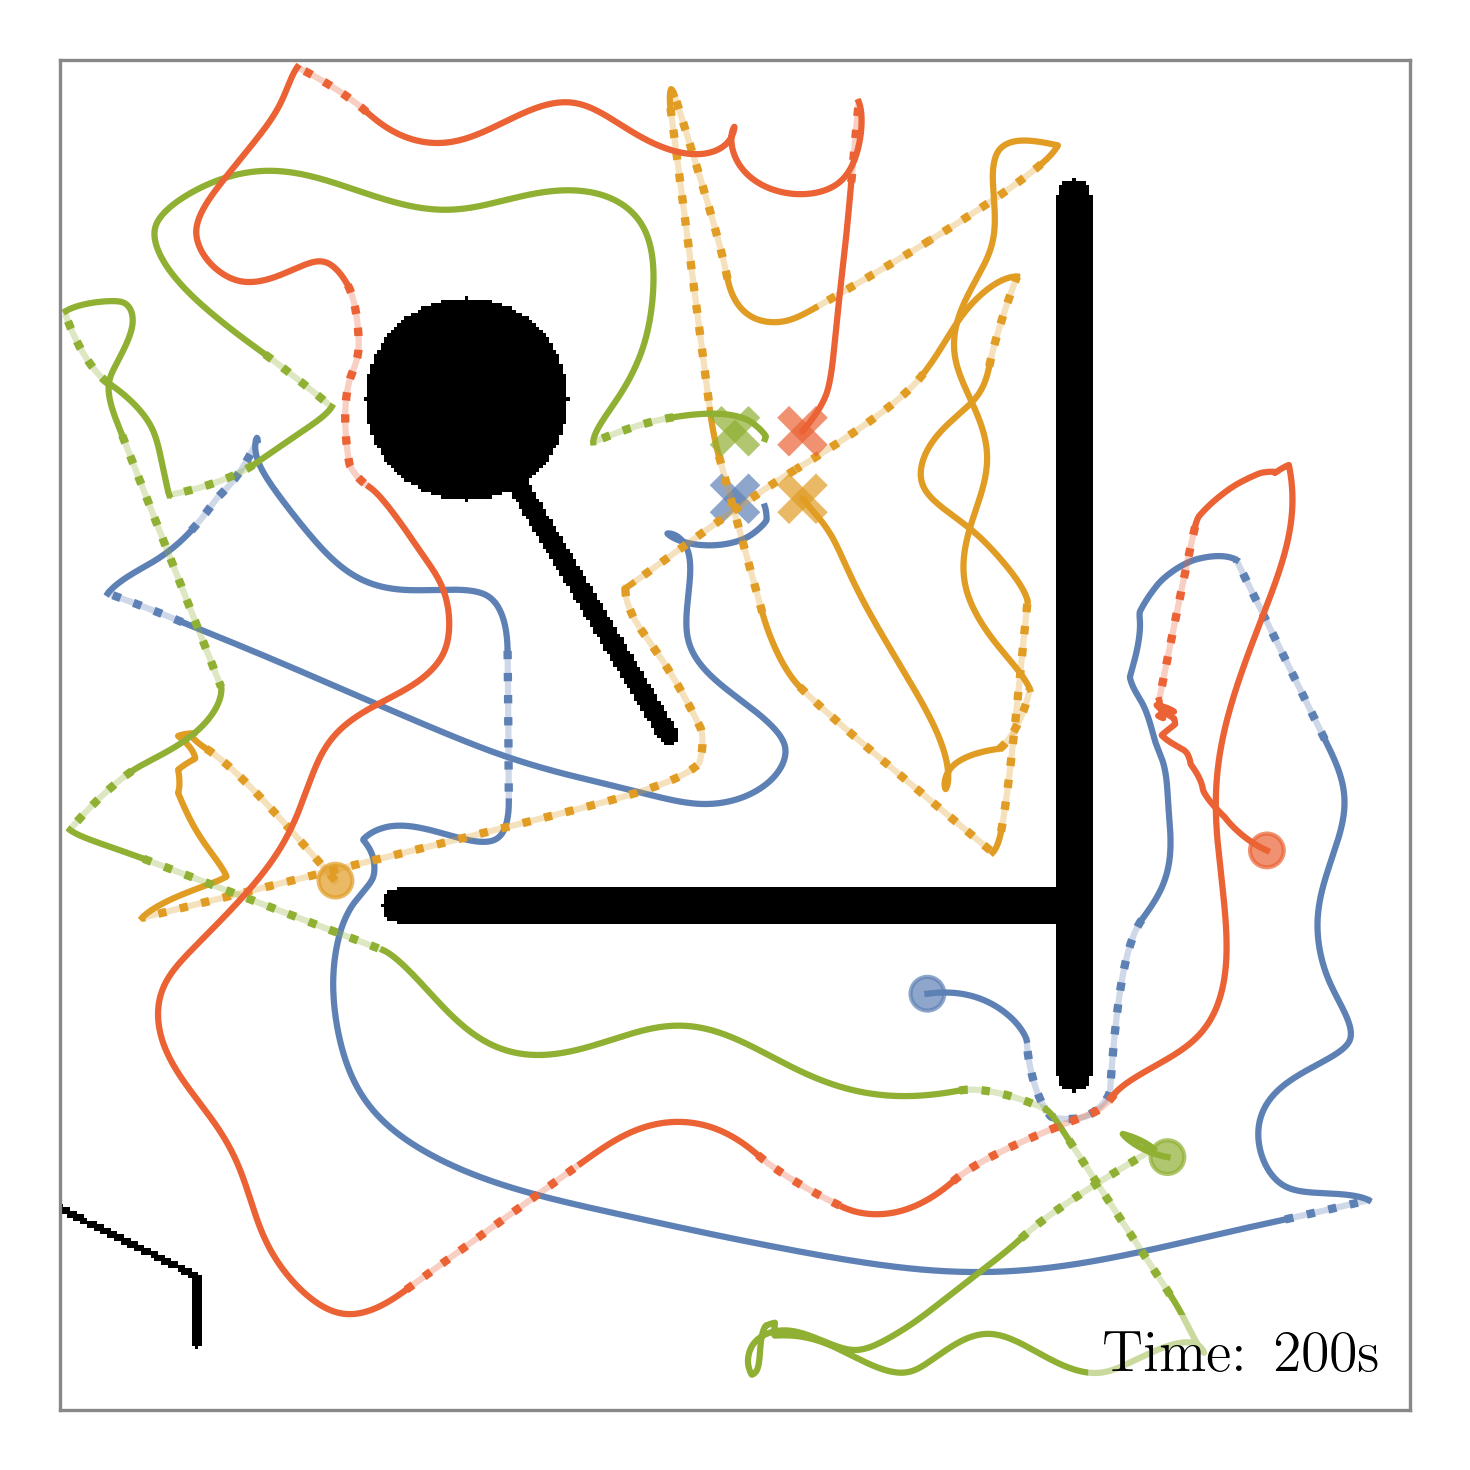
\includegraphics[width=\textwidth]{./figures/plots/paths/search:hybrid-paths-(after-200s).png}
    \end{subfigure}
    \begin{subfigure}[b]{\w}
        \centering
        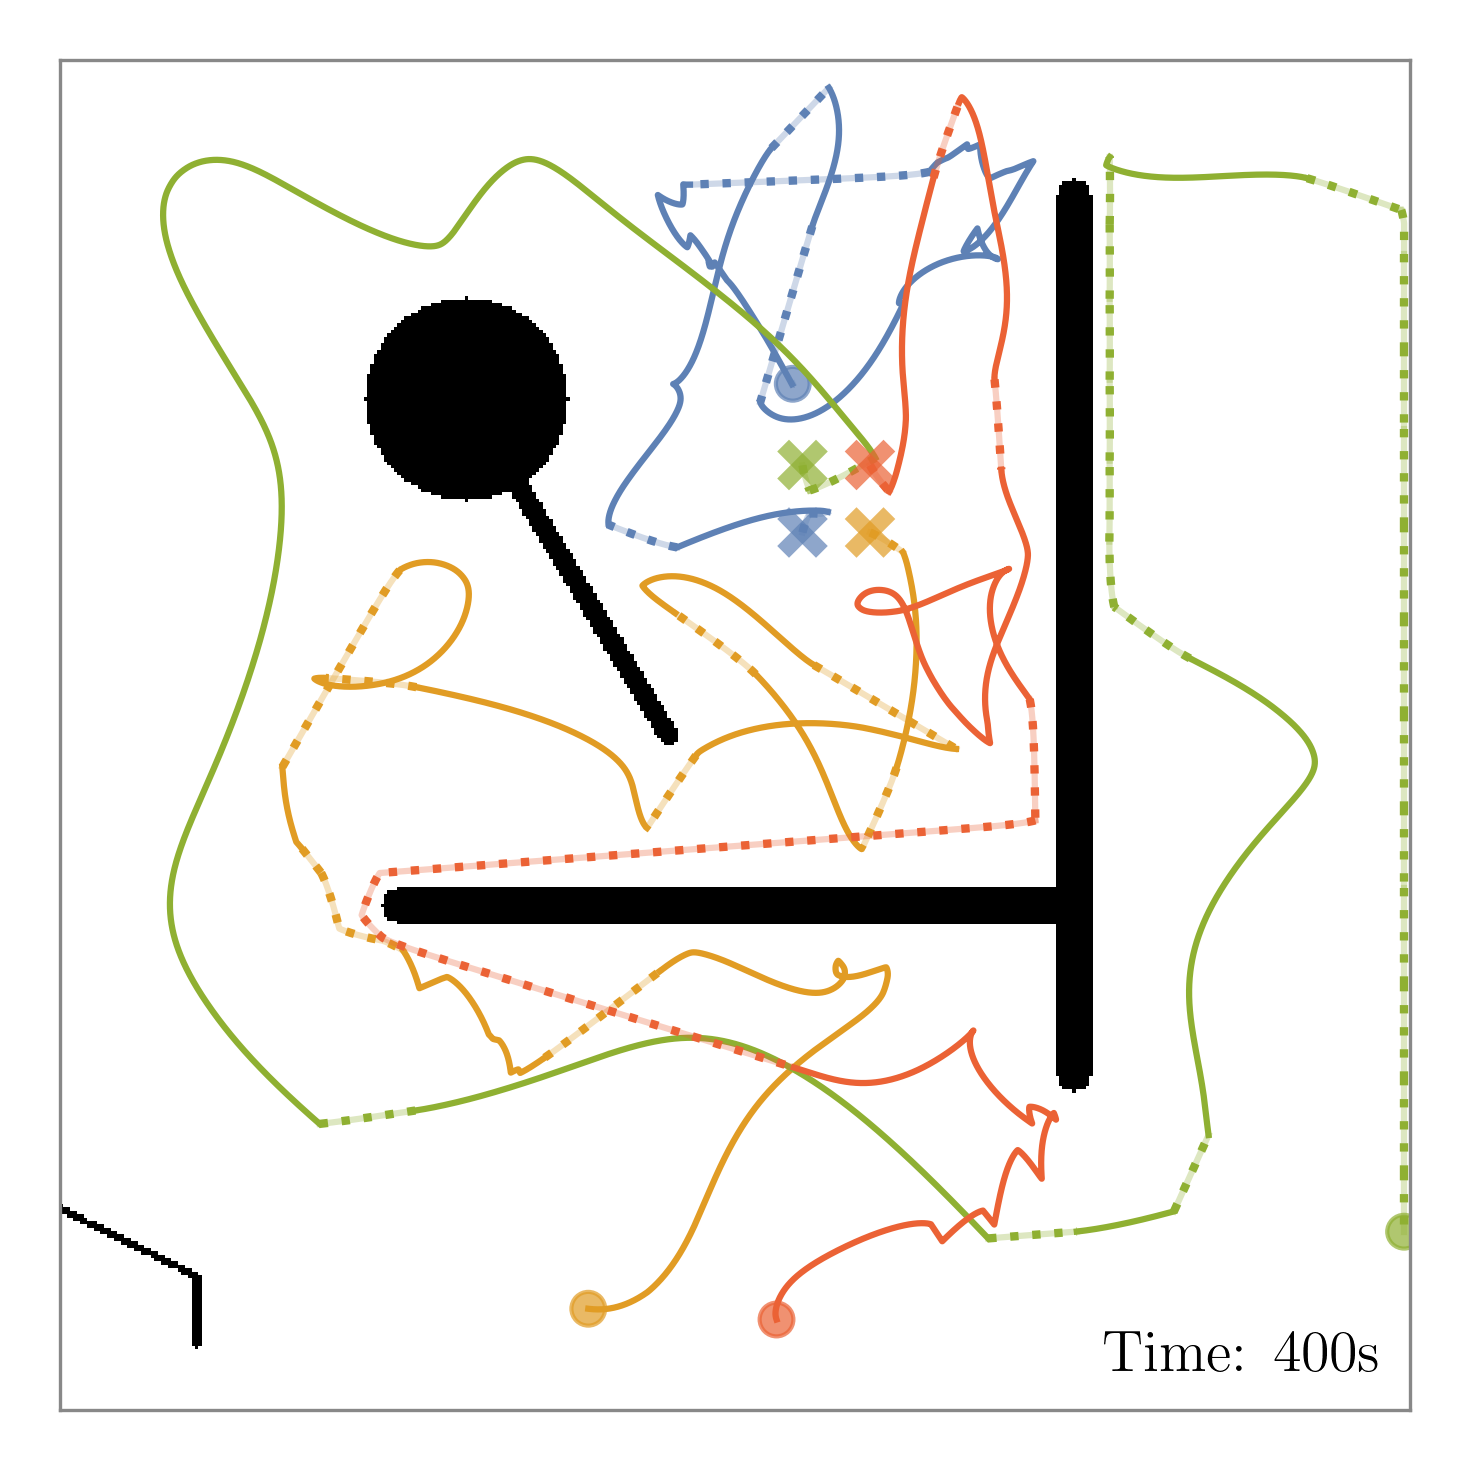
\includegraphics[width=\textwidth]{./figures/plots/paths/search:hybrid-paths-(after-400s).png}
    \end{subfigure}
    \begin{subfigure}[b]{\w}
        \centering
        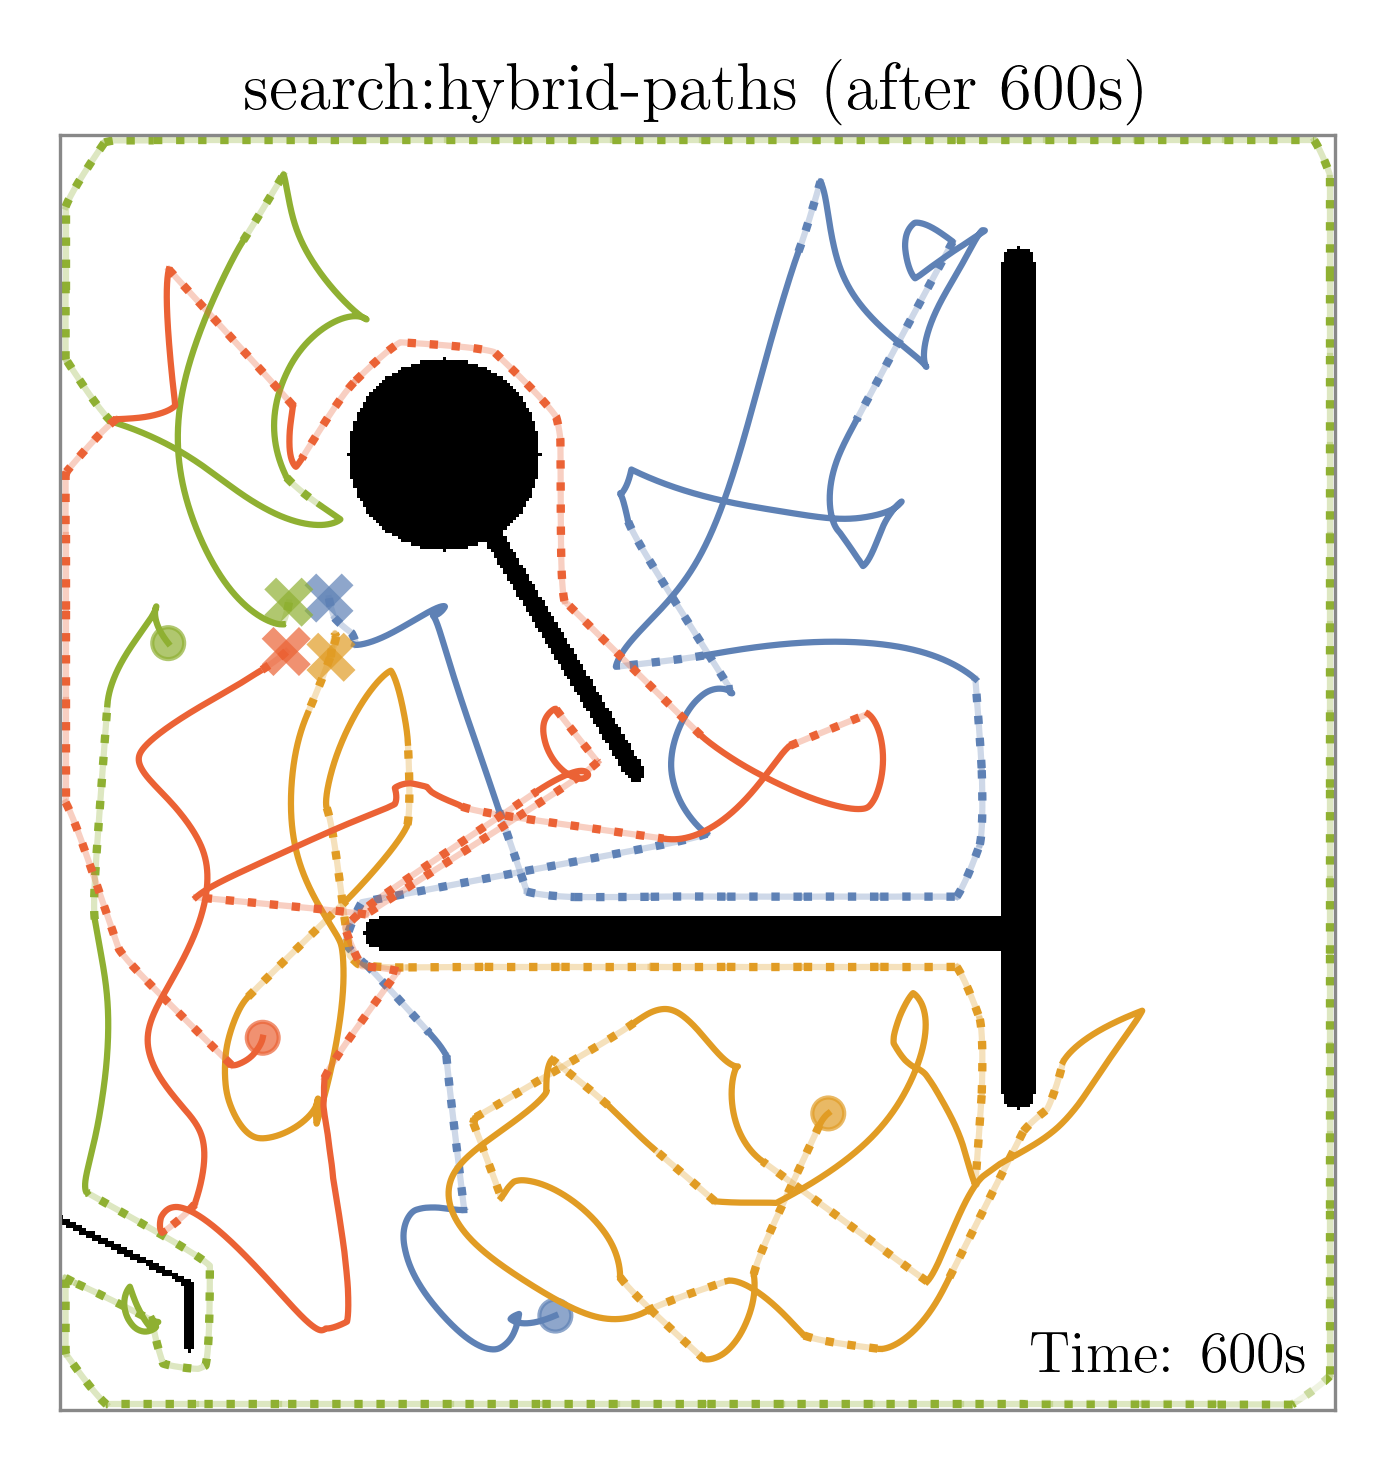
\includegraphics[width=\textwidth]{./figures/plots/paths/search:hybrid-paths-(after-600s).png}
    \end{subfigure}
    \caption{Paths of four robots running the hybrid algorithm after 200 s, 400 s, and 600 s in an example world simulated using \texttt{simple\_sim}. Solid lines indicate gradient-based motion, dashed lines path-following. Crosses mark starting positions, circles end positions.}
    \label{fig:hybrid-paths}
\end{figure}

\Cref{fig:hybrid-paths} shows the resulting behavior, where solid lines represent gradient-based movement and dashed lines indicate global path-following. This behavior produces a more spread out swarm as compared with the pure gradient-based algorithm which may lead to better search efficiency.

\subsection{Pure Pathing Algorithm}
An alternative to the hybrid approach is to use the global planner exclusively. In this case, the robot continuously alternates between selecting a new goal and following the computed path. \Cref{fig:pure-pathing-paths} shows example paths. As with the hybrid algorithm, the trajectories are smooth and consistent, with little lingering.

\def\w{0.329\textwidth}
\begin{figure}[H]
    \centering
    \begin{subfigure}[b]{\w}
        \centering
        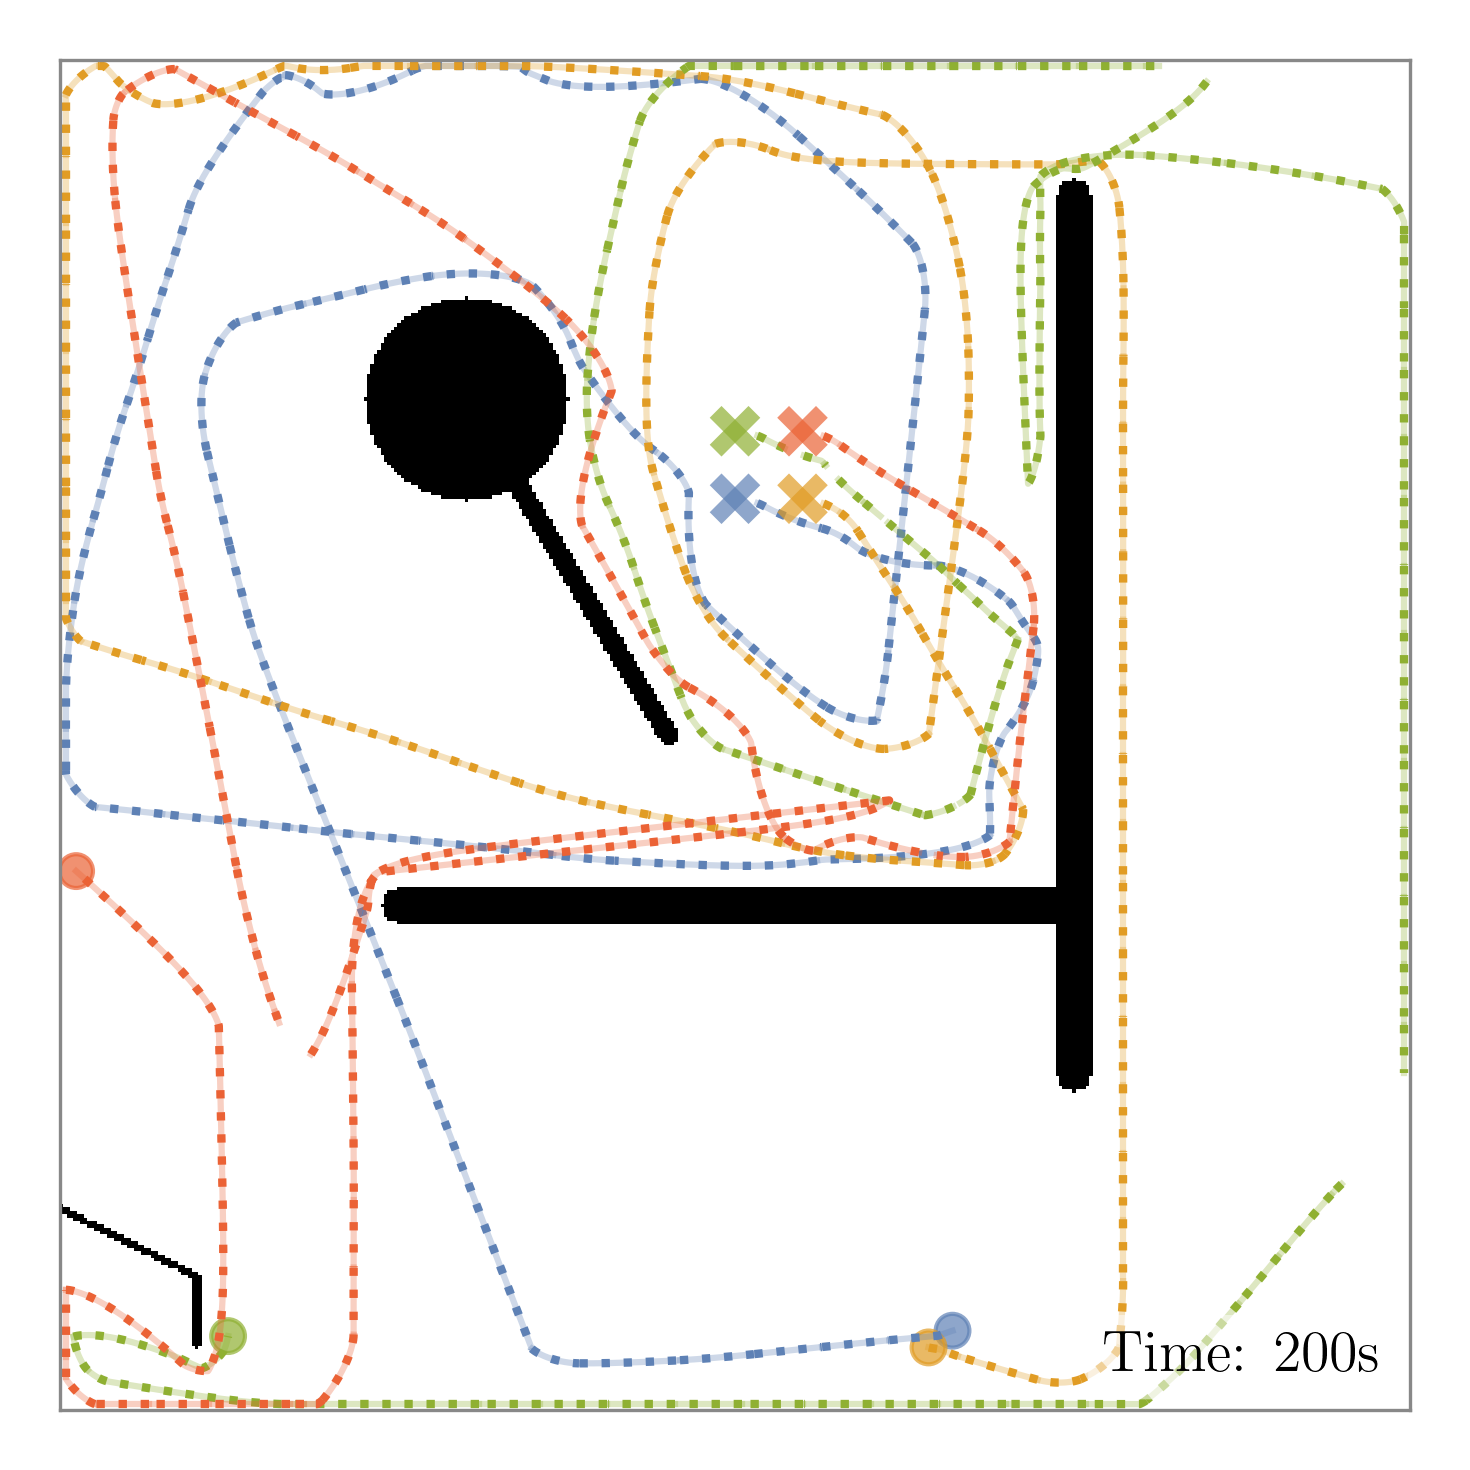
\includegraphics[width=\textwidth]{./figures/plots/paths/search:pathing-paths-(after-200s).png}
    \end{subfigure}
    \begin{subfigure}[b]{\w}
        \centering
        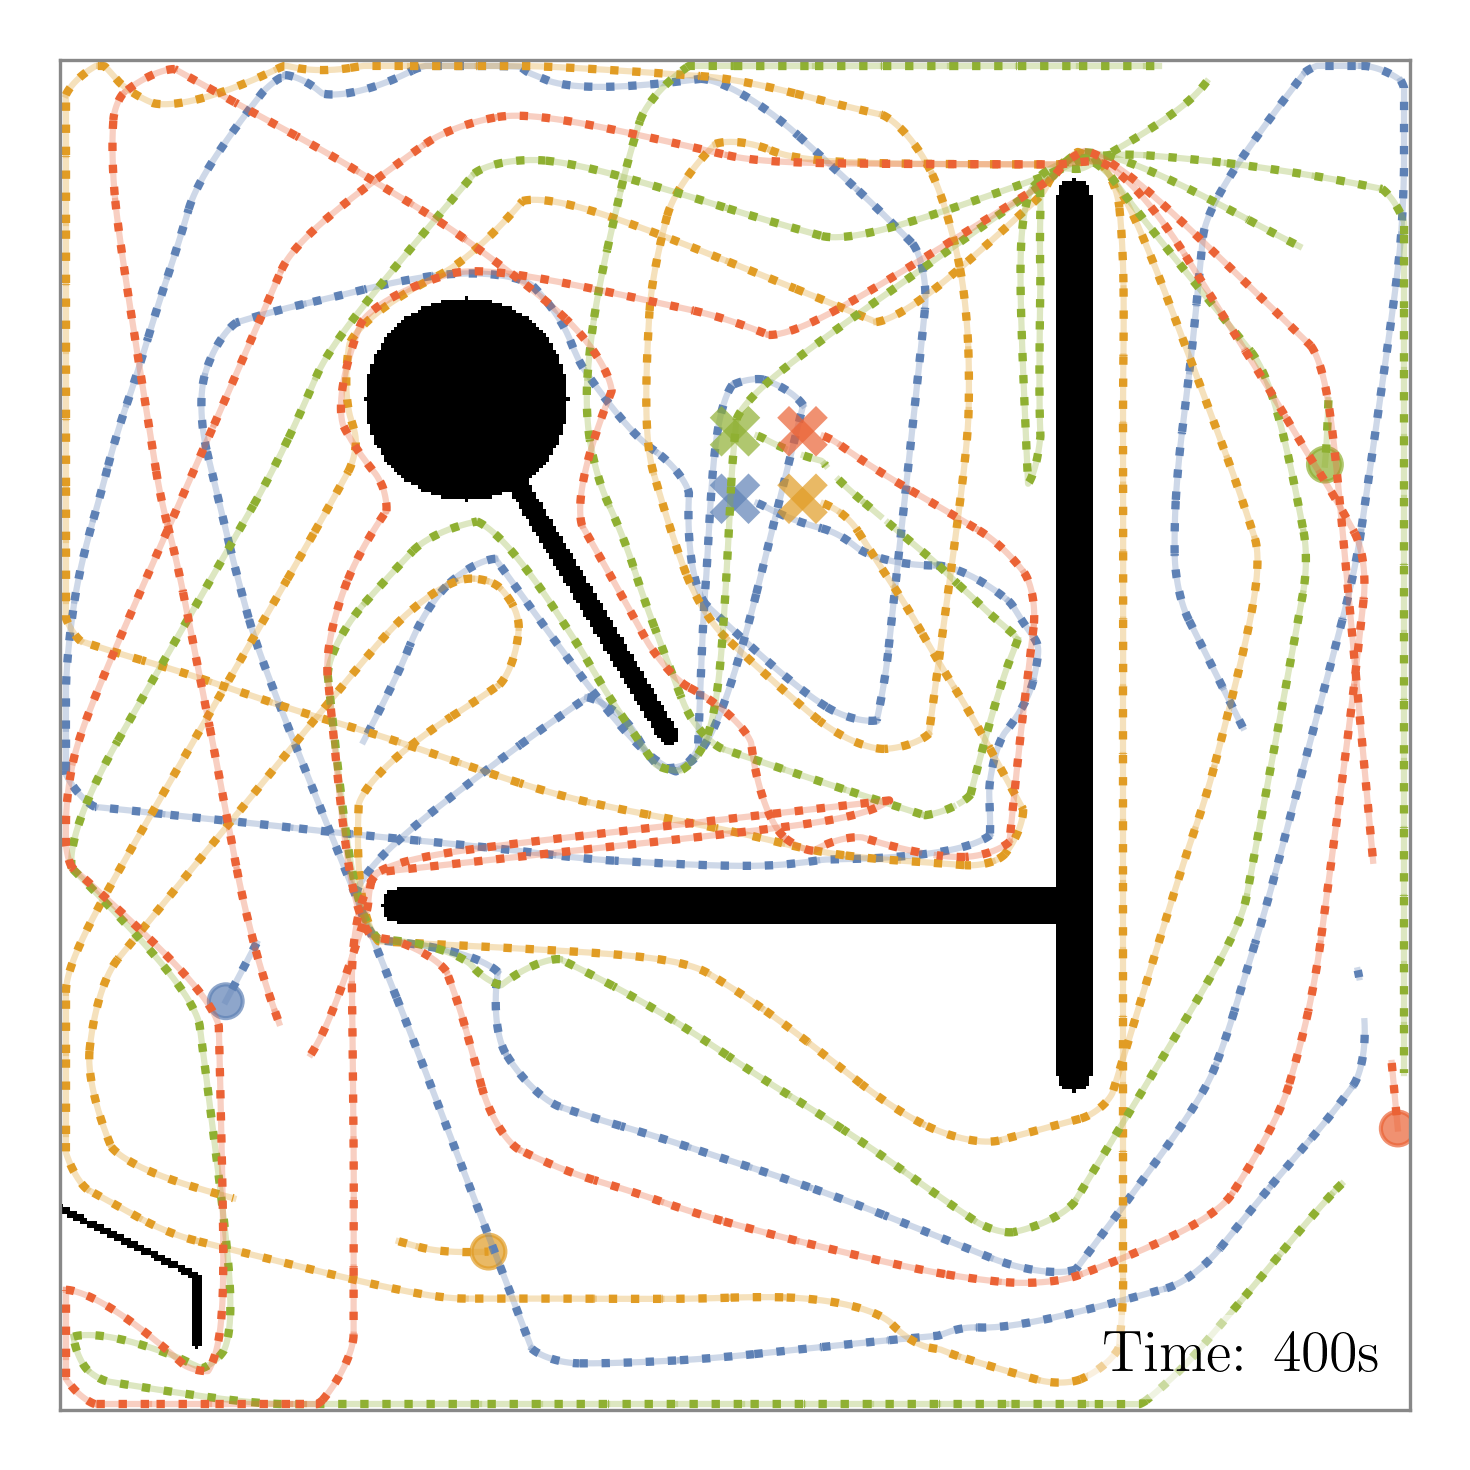
\includegraphics[width=\textwidth]{./figures/plots/paths/search:pathing-paths-(after-400s).png}
    \end{subfigure}
    \begin{subfigure}[b]{\w}
        \centering
        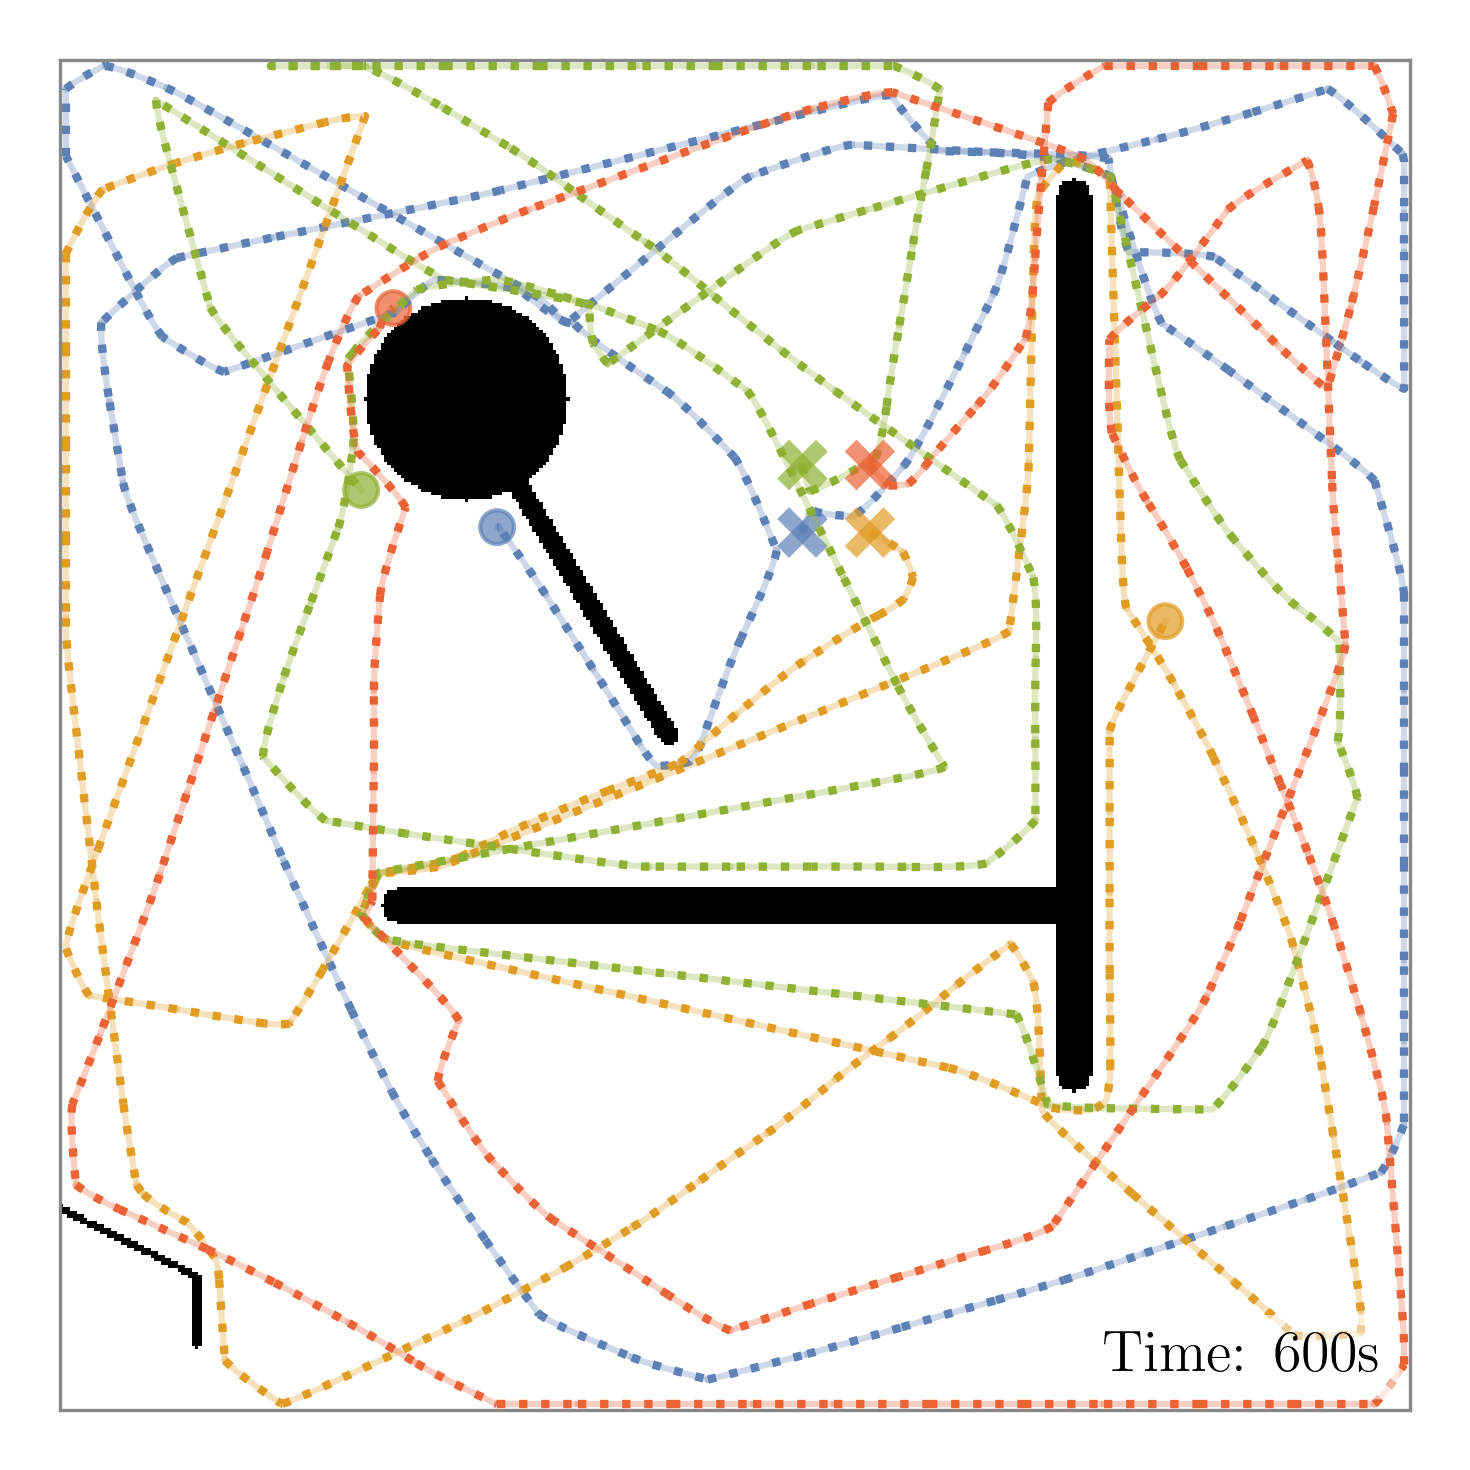
\includegraphics[width=\textwidth]{./figures/plots/paths/search:pathing-paths-(after-600s).png}
    \end{subfigure}
    \caption{Paths of four robots using the pure pathing algorithm. Dashed paths indicate full-time path-following. Crosses mark starting positions; circles indicate end positions.}
    \label{fig:pure-pathing-paths}
\end{figure}

The pure pathing algorithm also achieves full map coverage, with highly structured and efficient motion. A comparative analysis of all algorithms is presented in \cref{sec:results}.
